%%%%%%%%%%%%%%
% Fichero: uclmTFGesi.tex
% Autor: Jesús Salido Tercero (http://www.uclm.es/profesorado/jsalido)
% Fecha (creación): Febrero 2010
% Rev. : Febrero 2019
% Descripción: Plantilla para memoria de TFG
% (Escuela Sup. de Informática, UCLM). Creada para el curso
% “LaTeX esencial para preparación de TFG, Tesis y otros documentos
% académicos” (Esc. Sup. Informática-UCLM)
%
% Comentarios: Preparada para `pdflatex' y `biblatex'
% Documento editado con TeXstudio.
%%%%%%%%%%%%%%


% -------------------------
%
% PREÁMBULO del documento
%
% -------------------------

\newif\ifspanish%Definición de un condicional (spanish)

\spanishtrue 			% Idioma pral.: español (spanish=true)

\documentclass[ 		% Clase del documento
	11pt,				% Tamaño de letra
	a4paper,			% Tamaño de papel
	twoside,			% Impresión a doble cara
	openright,			% La apertura de cap. a la dcha.
	final       		% Versión final
]{book}

\usepackage[utf8]{inputenx} % Codificación de entrada
\usepackage[english,spanish,es-tabla,es-noindentfirst]{babel} % Internacionalización
\usepackage{indentfirst} % Para asegurar sangrado en 1ª línea tras sección (necesario con varios idiomas)

%--- Geometría de las páginas del documento
\usepackage[			% Márgenes del documento
	top=2.5cm,			% Margen superior
	bottom=2.5cm,		% Margen inferior
	inner=3.5cm,		% Margen al interior (Margen mayor debido a la encuadernacion. Asegurarse)
	outer=2cm			% Margen al exterior
]{geometry}


%--- Tipografía
\usepackage{textcomp,marvosym,pifont} % Generación de símbolos especiales
\usepackage{ccicons} % Iconos de licencia Creative Commons
\usepackage{amsmath,amsthm,amssymb}	% Mejoras cuando hay matemáticas
\usepackage{float} % Para posicionar las imagenes donde quiero
%--- Tipografía (Opción 1)
\usepackage[tt=false]{libertine}	% Libertine
\usepackage[libertine]{newtxmath}	% Times
%---

%--- Tipografía (Opción 2)
%\usepackage{newpxtext}				% Palatino: La opción osf proporciona números en old style.
%\usepackage{newpxmath}				% Palatino
%---


\usepackage[T1]{fontenc}% Codificación de salida
\usepackage{microtype}	% Mejoras de microtipografía en la obtención de PDF (sólo para pdflatex)


\usepackage{url} 		% Para escritura de URL
\urlstyle{sf}			% Estilo sans serif para URLs


%--- Definición de colores
% Este paquete debe cargarse antes de ctable.
% Revisar la documentación del paquete para ver los nombres de colores predefinidos.
\usepackage[%
	usenames,
	dvipsnames,
	svgnames,
	x11names,
	table
]{xcolor}


%--- Color especial definido para los hiperenlaces
\definecolor{palered}{rgb}{.8,0,0}


%--- Generación de hiperenlaces
\usepackage[
	pdftex,
	breaklinks,			% Permite que los links ocupen más de una línea
%	hidelinks,			% Oculta el color y borde de los links
% OJO: La opción colorlinks se comenta para evitar un error con el paquete menukeys.
%	colorlinks=true,	% Pone color en los link o un borde
	linkcolor=palered,	% Color de los links
	anchorcolor=palered,
	citecolor=palered,
	filecolor=palered,
	menucolor=palered,
	urlcolor=palered,
	bookmarksnumbered=true % Incluye números en bookmarks
]{hyperref}


\usepackage{pdfpages}  % Permite inclusión de páginas de un PDF


%--- Paquetes para listas y organización de texto
\usepackage{paralist}	% Mayor control de listas
\usepackage{multicol}	% Texto en varias columnas


%--- Gráficos y tablas
\usepackage{graphicx}	% Inclusión de figuras
\usepackage{subfigure}	% Inclusión de subfiguras
% EDITAR: Si es necesario cambiar el path para los directorios de figuras.
\graphicspath{{./figs/}}% Path de búsqueda de ficheros gráficos
\DeclareGraphicsExtensions{.pdf,.png,.jpg} % Precedencia de extensiones
\usepackage{rotating}	% Giro de cajas (texto, figuras, tablas) (No DVI)
\usepackage{tabularx,booktabs}	% Ajustes para tablas


%--- Paquetes especiales para Informática
\usepackage{listings}	% Inclusión de listados de código




%--- Personalización de títulos de figuras y tablas
\usepackage[%
	margin=10pt,		% Margen
	font=small,			% Tamaño de tipografía
	labelfont=bf,		% Prefijo-Etiqueta en negrita
	format=hang			%
]{caption}
\captionsetup[table]{skip=4pt} 	% Separación del caption en las tablas
\usepackage{eurosym} % para el euro
%--- Bibliografía: Biblatex con biber.
% OJO: Para bib multilingüe añadir campos language y langid en registros bib.
\usepackage[
	backend=bibtex, 		% Backend
	sortcites,
	defernumbers=true, 	% Para numerar al final
	style=numeric-comp, % Estilo numérico condensado
	autolang=other, 	% Requerido para opción multilingüe
	language=auto   	% Requerido para opción multilingüe
]{biblatex}


% Línea añadida para eliminar el idioma de la fuente bibliográfica.
\AtEveryBibitem{\clearfield{note} \clearlist{language}}
\addbibresource{biblioTFG.bib} 	% Fichero de bibliografía.
\usepackage[autostyle]{csquotes}
%---



%--- Paquete con personalización local para el TFG (ESI-UCLM)
\usepackage{uclmTFGesi}
% -------------------------
% PAQUETES QUE USA:
% 	fancyhdr,titlesec,sectsty,tikz
% -------------------------
% LISTA DE COMANDOS PROPORCIONADOS:
% OB-Obligatorio
% OP-Opcional
% RE-Recomendado
%
% Comandos para definir variables con los datos del documento.
%
% OB-\portadaTFG				: Pág. de portada (usa variables definidas)
% OB-\portadillaTFG				: Pág. de portada interna
% OB-\tribunalTFG				: Pág. tribunal
% RE-\dedicado{texto}			: Pág. de dedicatoria con texto
% RE-\creditos{texto}{imagen}	: Pág. de créditos con el texto y la imagen
% OB-\abstract{texto}			: Añade abstract (no definido en clase book)
% OP-\tecla{texto}				: Borde de tecla en torno al texto (sustituir por menukeys)
% OP-\nodivide[penalty]			: Penaliza la división de palabras.
%								  Máx. (n=10000) sin arg.
% OP-\nowidowandorphan[penalty]: Penaliza las viudas y huérfanas.
%								(sólo si necesario)
% OP-\nodividenotes[penalty]	: Penaliza la división de notas al pié
%								entre págs.	(sólo si necesario)
% OP-\savepagecnt				: Crea contador interno con el nº de pág. actual
% OP-\contpagination			: Recupera el valor de pág. previamente
%								 salvado en el cont. interno.
% RE-\cleanhdfirst				: Elimina la cabecera en la primera
%								página de capítulo.
%
% -------------------------




%--- Paquete para índice temático
\usepackage{makeidx}
\makeindex


%--- Paquete para incluir menús, paths y teclas de modo "elegante"
% OJO: Este paquete presenta algunas incompatibilidades, debe cargarse el último y exige la desactivación de la opción colorlinks y la inclusión en este paquete de la opción hyperrefcolorlinks.
% Este paquete presenta alguna incompatibilidades por lo que cambiarlo de ubicación puede generar algún error (manejar con cuidado).
\usepackage[os=win,hyperrefcolorlinks]{menukeys}

% Estas definiciones permiten cambiar el estilo de los elementos. Si se desean otros estilos o su configuación es preciso recurrir a la documentación del paquete (no lo recomiendo).
\renewmenumacro{\menu}[>]{menus} % default: menus
\renewmenumacro{\directory}[/]{pathswithblackfolder} % default: paths
\renewmenumacro{\keys}[+]{shadowedroundedkeys} % default: roundedkeys

%%%%%%%%%%%%%%%%%%%%%%%%%%%%%%%%%%%%%%%%%%%%%%%%%%%%%
%%%%%%%%%%%%%%%%%%%%%%%%%%%%%%%%%%%%%%%%%%%%%%%%%%%%%
%%%%%%%%%%%%%%%%%%%%%%%%%%%%%%%%%%%%%%%%%%%%%%%%%%%%%





% -------------------------
%
% DATOS DEL DOCUMENTO
% Definición de variables empleadas en el documento por lo que no son
% traducidos. Cuando algún campo puede tener varias líneas aparecen dos
% campos señalados como <campo>Primera y <campo>Segunda.
% Si no se desea emplear un campo este debe comentarse.
%
% -------------------------
% Datos del documento
\tituloPrimera{Sistema Inteligente para la Gestión y Optimización de Energía basado en la Nube}	% 1ª Línea
%\tituloSegunda{} % 2ª Línea
\titulo{Sistema Inteligente para la Gestión y Optimización de Energía basado en la Nube}
\autor{Pablo Palomino Gómez}
\email{pablo.palomino1@alu.uclm.es}
\director{Luis Jiménez Linares}
\codirector{Luis Rodríguez Benítez}
\instEdu{UNIVERSIDAD DE CASTILLA-LA MANCHA}
% Fichero con escudo de la institución
% Poner el logo del centro que corresponda
%\escudo{esi}
%\escudo{esicolor}
%\escudo{logo_ESI}
\escudo{escudoInf} 	% Nucleo de ferrita
%\escudo{uclm}
%\escudo{etsii}

\centroEdu{ESCUELA SUPERIOR DE INFORMÁTICA}
\deptoEduPrimera{Departamento de Tecnologías y Sistemas de Información}% 1ª Línea
%\deptoEduSegunda{<Segunda línea Depto. Director>}% 2ª Línea
\titulacion{GRADO EN INGENIERÍA INFORMÁTICA}
\especialidad{TECNOLOGÍA ESPECÍFICA DE COMPUTACIÓN}
\tipoDoc{TRABAJO FIN DE GRADO}
% Si las fechas se desean en inglés hay que ponerlas explícitamente.
\fechaDef{Julio, 2019} 							% Fecha de defensa
\mesDef{Julio}        							% Mes de defensa
\yearDef{2019}        							% Año de defensa
\lugarDef{Ciudad Real}							% Lugar de defensa


% --- Propiedades para el documento PDF
\hypersetup{
	pdftitle={TFG\_PalominoGomezPablo}, % Título
	pdfauthor={P. Palomino},                        	% Autor
	pdfsubject={TFG},					% Tema
	pdftoolbar=true,					% Muestra la toolbar de Acrobat
	pdfmenubar=true						% Muestra la menubar de Acrobat
}
% -------------------------

%--- Acrónimos
\usepackage[acronym,nomain,nonumberlist,toc]{glossaries}
\newglossaryentry{TFG}{name=TFG, description={Trabajo fin de grado}}
\newglossaryentry{CMP}{name=CMP, description={\textit{Current module power}}}
\newglossaryentry{API}{name=API, description={\textit{Application Programming Interface}}}
\newglossaryentry{AEMET}{name=AEMET, description={Agencia estatal de meteorlogía}}
\newglossaryentry{REE}{name=REE, description={Red eléctrica de España}}
\newglossaryentry{PVPC}{name=PVPC, description={Precio voluntario al pequeño consumidor}}
\newglossaryentry{JSON}{name=JSON, description={\textit{JavaScript object notation}}}
\newglossaryentry{PSR}{name=PSR, description={Problema de satisfacción de restricciones}}
\newglossaryentry{EF}{name=EF, description={Variable de energía fotovoltaica}}
\newglossaryentry{ER}{name=ER, description={Variable de energía de red}}
\newglossaryentry{EB}{name=EB, description={Variable de energía de batería}}
\newglossaryentry{CB}{name=CB, description={Variable de consumo de batería}}
\newglossaryentry{CR}{name=CR, description={Variable de consumo de red}}
\newglossaryentry{WSGI}{name=WSGI, description={\textit{Web server gateway interface}}}
\newglossaryentry{PaaS}{name=PaaS, description={\textit{Platform as a service}}}
\newglossaryentry{IaaS}{name=IaaS, description={\textit{Infrastructure as a service}}}
\newglossaryentry{AWS}{name=AWS, description={\textit{Amazon web services}}}
\newglossaryentry{EC2}{name=EC2, description={\textit{Amazon elastic compute cloud}}}
\newglossaryentry{XP}{name=XP, description={\textit{Extreme programming}}}
\newglossaryentry{GLP}{name=GNU GLP, description={Licencia pública general de GNU}}

\makeglossaries

% -------------------------
%
% CUERPO DEL DOCUMENTO
%
% -------------------------
\begin{document}

%--- Ajustes del documento (en páginas iniciales).
\ifspanish
	\selectlanguage{spanish}% Emplea idioma español
\else
	\selectlanguage{english}% Emplea idioma inglés
\fi

\frontmatter
% Cambia la numeración de páginas a números romanos y las secciones no están numeradas aunque si aparecen en el índice de contenidos.
\pagestyle{empty}  % Páginas sin cabecera ni pies
%---



% -------------------------
%
% PORTADAS
%
% -------------------------
\portadaTFG		% Portada pral.

\portadillaTFG	% Portada interior (añade tutores)
%---

% -------------------------
%
% CRÉDITOS
%
% -------------------------
% Este comando permite una gran flexibilidad y la ventaja de no depender de paquetes externos.
% Esta es una página reservada para señalar información relativa a los derechos de autor y la licencia de distribución y uso del documento. Esta página debería ser aprovechada también para informar de cualquier tipo de cesión de los derechos anteriormente citados. El autor del TFG debe tener presente que el incumplimiento de la legislación vigente en materia de protección de la propiedad intelectual es de su exclusiva responsabilidad independientemente de la cesión de derechos que este haya convenido para su obra ya que no son objeto de cesión aquellos derechos de los que no se es poseedor.

\creditos{Este documento se distribuye con licencia Creative Commons Atribución Compartir Igual 4.0. El texto completo de la licencia puede obtenerse en \url{https://creativecommons.org/licenses/by-sa/4.0/}.
% El escudo de Informática basado en el nuclo de ferrita que acompaña la distribución de esta plantilla ha sido realizado por P.~Moya, D.~Villa e I. Díez, su inclusión debe respetar los derechos de autor y las licencias a las que se vea sometido.

La copia y distribución de esta obra está permitida en todo el mundo, sin regalías y por cualquier medio, siempre que esta nota sea preservada. Se concede permiso para copiar y distribuir traducciones de este libro desde el español original a otro idioma, siempre que la traducción sea aprobada por el autor del libro y tanto el aviso de copyright como esta nota de permiso, sean preservados en todas las copias.\\}{cclicense}
%---

% -------------------------
%
% TRIBUNAL
%
% -------------------------
\tribunalTFG % Página para calificaciones del tribunal
%---


% -------------------------
%
% DEDICATORIA (opcional, 1 pág. máximo)
% Aunque opcional, no se debería perder la oportunidad de poder
% dedicar el trabajo a alguien MUY especial.
%
% -------------------------
% EDITAR: Dedicatoria (comentar si no se desea incluir).
\dedicado{A mis padres, por inculcarme el valor del esfuerzo\\ A Nuria, por potenciarlo}
%---









%--- Ajustes del documento.
\pagestyle{plain}	% Páginas sólo con numeración inferior al pie

% -------------------------
%
% RESUMEN:
% OJO: Si es preciso cambiar orden manualmente
%
% -------------------------
%--- Resumen en español
\selectlanguage{spanish} % Selección de idioma del resumen.
\cleardoublepage % Se incluye para modificar el contador de página antes de añadir bookmark
\phantomsection  % OJO: Necesario con hyperref
\pdfbookmark[0]{Resumen}{idx_resumen}% idx_resumen.0 % Bookmark en PDF


\begin{abstract}
El consumo de energía juega un papel fundamental en el progreso y bienestar de la sociedad. Tanto es así que la demanda de energía se multiplica con el paso del tiempo y por lo tanto, el precio de la misma. Además, las fuentes de energía fósiles son agotables y se debe ir apostando por medios de extracción de energías renovables tanto como sea posible. Para poder lidiar con ello se debería poder obtener energía de numerosas fuentes, dependiendo de varios factores que las condicionan y seleccionando la más adecuada en cada momento, sin depender de una única fuente energética para satisfacer la demanda como ocurre actualmente. Lamentablemente esto es ardúa tarea para el ser humano, pero alcanzable para la computación.\\

Este trabajo fin de grado consiste en la creación de un sistema inteligente para la gestión de energía en el hogar de la manera más óptima y eficiente posible. En función de un escenario determinado en cada hora del día, el sistema es capaz de modelar la cantidad de energía eléctrica recibida por cada una de las fuentes de entrada energética para realizar el menor gasto económico posible en su obtención. De igual modo, el sistema modela la cantidad de energía eléctrica suministrada a una serie de salidas, pues toda la energía generada debe ser consumida de uno u otro modo, como puede ser el consumo del hogar, carga de una batería, etc. Esto se traduce en una optimización y aprovechamiento de la energía, que además tiene como consecuencia un ahorro económico en la obtención de la energía necesaria. Para hacer esto posible se modela un problema de satisfacción de restricciones (PSR) cuyas soluciones son alcanzadas mediante programación lineal, haciendo uso de algoritmos de computación científica. Además, consta de una aplicación web que permite realizar simulaciones de optimizaciones diarias a sus usuarios, alojada en la nube de IBM Cloud Foundry y Amazon Web Services.

\end{abstract}
%---

%--- Resumen en inglés
% Abstract
\selectlanguage{english}
\cleardoublepage
\phantomsection % OJO: Necesario con hyperref
\pdfbookmark[0]{Abstract}{idx_abstract}% idx_abstract.0 % Bookmark en PDF

\begin{abstract}
Energy consumption plays an essential role in the development and well-being of society. The demand for energy multiplies over time and thus the price of energy. Furthermore, fossil energy sources are exhaustible and we must opt for the means of extracting renewable energies as much as possible. In order to be able to deal with this, it should be possible to obtain energy from different sources, depending on various factors that condition them and selecting the most appropriate one at each moment, without depending on a single energy source to satisfy demand as is currently happens. Unfortunately this is a difficult task for the human being, but possible for computing.\\

This project is focused on the creation of an intelligent system for managing energy in the home in the most optimal and efficient way possible. Depending on a given situation at each hour of the day, the system is able to model the amount of electrical energy received by each energy input sources to make the lowest economic cost in obtaining it. At the same time, the system models the amount of electrical energy supplied to a series of outputs, as all the energy generated must be consumed in one way or another, such as home consumption, charging a battery, etc.. This can be translated into an optimization and use of energy, which also results in economic savings in obtaining just the required energy. In order to make this possible, a constraint satisfaction problem (CSPs) is modeled, the solutions of this CSPs are reached by means of linear programming, making use of scientific computing algorithms. In addition and in order to allow users to perform highly precise simulations for daily optimizations, a web application was developed within this project. This application is hosted in the cloud, using modern cloud services like IBM Cloud Foundry and Amazon Web Services.
\end{abstract}
%---

% Selección de idioma para el resto del documento y adaptación de títulos de sección.
% EDITAR: Sólo si es necesario.
% NOTA: Al cambiar de idioma las def. de títulos se reinician.
\ifspanish
	\selectlanguage{spanish}% Para el resto del documento el idioma es español.
	%--- No necesarios al añadir la opción es-tabla para babel.
	%\renewcommand{\tablename}{Tabla} % Se sustituye 'Cuadro' por 'Tabla'
	%\renewcommand{\listtablename}{Índice de tablas}
	%---
	\renewcommand{\lstlistingname}{Listado}
	\renewcommand{\lstlistlistingname}{Índice de listados}
	% Modififica las macros \algorithmcfname y \listalgoritmcfname
	\renewcommand{\appendixname}{Anexo}
	\renewcommand{\bibname}{Bibliografía}
	\renewcommand{\indexname}{Índice temático}
\else
	\selectlanguage{english}
\fi

% -------------------------
%
% AGRADECIMIENTOS (recomendable máx. 1 pág.)
%
% -------------------------
\cleardoublepage
\phantomsection % OJO: Necesario con hyperref
\pdfbookmark[0]{Agradecimientos}{idx_agrad}% idx_agrad.0 % Bookmark en PDF

\chapter*{Agradecimientos} % Opción con * para que no aparezca en TOC ni numerada

%OJO: Editar
 Aunque es un apartado opcional, haremos bueno el refrán \emph{<<Es de bien nacidos, ser agradecidos>>} si empleamos este espacio es un medio para agradecer a todos los que, de un modo u otro, han hecho posible que el TFG <<llegue a buen puerto>>. Esta sección es ideal para agradecer a familiares, directores, profesores, compañeros, amigos, etc. 
 
 Estos agradecimientos pueden ser tan personales como se desee e incluir anécdotas y chascarrillos, pero nunca deberían ocupar más de una página.

\makeatletter		
\begin{flushright}
	\textit{\@autor}
\end{flushright}
\makeatother % Agradecimientos etc.




% -------------------------
%
% ÍNDICES
%
% -------------------------
\pagestyle{fancy} % Estilo de página ajustado por fancyhdr

% EDITAR: Si alguno de los índices no existe, su inclusión se puede comentar.
\cleardoublepage
\phantomsection % OJO: Necesario con hyperref
\pdfbookmark[0]{Índice general}{idx_toc}% idx_toc.0 % Bookmark en PDF

\tableofcontents  % Índice general

% Todos los listados se han incluido en el índice de contenidos. De modo automático también quedan añadidos a los bookmarks del PDF. Si se desean eliminiar del TOC se pueden comentar el comando \addcontensline.

\cleardoublepage
\phantomsection % OJO: Necesario con hyperref
\addcontentsline{toc}{chapter}{\listfigurename} % Añade la lista de figuras al TOC (también a bookmarks en PDF)
%\pdfbookmark[0]{\listfigurename}{idx_lof}% idx_lof.0 % Bookmark en PDF
\listoffigures    % Índice de figuras (opcional)

\cleardoublepage
\phantomsection % OJO: Necesario con hyperref
\addcontentsline{toc}{chapter}{\listtablename} % Añade la lista de tablas al TOC (también a bookmarks en PDF)
%\pdfbookmark[0]{\listtablename}{idx_lot}% idx_lot.0 % Bookmark en PDF
\listoftables % Índice de tablas (opcional)

\cleardoublepage
\phantomsection % OJO: Necesario con hyperref
\addcontentsline{toc}{chapter}{\lstlistlistingname} % Añade la lista de listados al TOC (también a bookmarks en PDF)
%\pdfbookmark[0]{\lstlistlistingname}{idx_lol}% idx_lol.0 % Bookmark en PDF
\lstlistoflistings % Índice de listados creados con listings (opcional)

\cleardoublepage
\phantomsection % OJO: Necesario con hyperref
%\addcontentsline{toc}{chapter}{\listalgorithmcfname} % Añade la lista de algoritmos al TOC (también a bookmarks en PDF)
%\pdfbookmark[0]{\listalgorithmcfname}{idx_loa}% idx_loa.0 % Bookmark en PDF

\cleardoublepage
\phantomsection % OJO: Necesario con hyperref
\printglossary[title={Listado de acrónimos}]




























%--- MAINMATTER
% Capítulos del documento
% Salva en un contador interno el nº de páginas actual
% Debe ir antes de \mainmatter (antes de que se reinicie el cnt page)
\savepagecnt
\mainmatter
% Justo antes del primer capítulo del libro. Activa la numeración con números arábigos y reinicia el contador de páginas.

% OJO: No cambiar de ubicación. Elimina cabecera y pie en pág. inicial de cap.
\cleanhdfirst

% Reajuste del número de página consecutivo para no reiniciar paginación en Cáp. 1
%\contpagination % Comentado para reiniciar paginación (pag. 1)




% -------------------------
%
% CAPÍTULOS
%
% -------------------------
% Se incluye un fichero para cada capítulo. Se emplea la instrucción \include porque en los libros lo más habitual es que cada cápítulo comience en una nueva página.
\chapter{Introducción}
\label{cap:Introduccion}
El consumo de energía juega un papel muy importante en el progreso y bienestar de la sociedad. Tanto es así, que la demanda energética no deja de crecer, por ello deben llevarse a cabo medidas para reducir el consumo elevado de energía, lo que se conoce como eficiencia energética. La eficiencia energética~\cite{GarSa12} se refiere al empleo de medios de optimización en la producción y aprovechamiento de la energía, con el objetivo de proteger el medio ambiente. Esto ha pasado a ser una necesidad debido a que las emisiones de $ CO_{2} $ van en aumento y el cambio climático es un hecho.  \\

Por otro lado, puesto que las fuentes de energía fósil y nuclear son finitas, podría llegar el día en el que no se pueda satisfacer la demanda energética, salvo que se apueste por los métodos alternativos de obtención de energía. Es aquí donde entran en juego las energías renovables. Una de ellas es la energía solar~\cite{Perp12}, que permite el aprovechamiento de la radiación electromagnética del sol. Resulta interesante su estudio, debido a que es tan abundante que se considera inagotable: la cantidad de energía que el Sol vierte diariamente sobre la Tierra es diez mil veces mayor que la consumida al día en todo el planeta. Finalmente, además de ser una energía inagotable, es una energía limpia, una muy buena alternativa a los combustibles fósiles o energía nuclear. \\

Teniendo en cuenta estos dos antecedentes, existe una motivación a la hora de obtener la energía demandada de la forma mas óptima y limpia posible. Además, también debe tenerse en cuenta el factor económico. Actualmente la mayoría de particulares tienen una única fuente de suministro de energía que vendría a ser la compañía eléctrica de la cuál son clientes, importando la totalidad de la energía que su hogar demanda a dicha compañía, a un precio establecido PVPC~\cite{Ree14} (Precio voluntario al pequeño consumidor) que representa el precio máximo de referencia que pueden contratar los consumidores con hasta 10 Kwh de potencia contratada. Su valor tiene una discriminación horaria, lo que hace que en las horas de mayor consumo el precio sea mas alto. Sería interesante poder reducir la cantidad de energía que se obtiene de esta fuente en las horas pico (horas de máximo consumo donde el PVPC suele alcanzar el valor alto) y obtenerla de otra fuente cuyo precio sea menor, para así obtener un promedio mucho mas barato que con una única fuente de energía. Esto se puede lograr añadiendo nuevas fuentes al hogar, como puede ser la instalación de placas fotovoltaicas. Visto así parece muy sencillo y demasiado bueno para ser cierto, pero en el año 2015 mediante el Real Decreto 900/2015~\cite{Boe15} se establecieron unas condiciones para la instalación de placas fotovoltaicas, lo que se conoce coloquialmente como el "impuesto al sol". Por suerte, para potencias contratadas no superiores a 10 Kwh, no se pasa este impuesto, así que no es problema para el desarrollo y aplicación del sistema. Para tener el mínimo gasto posible, habría que obtener la cantidad óptima de cada una de las fuentes en cada momento, lo que supone un oficio tedioso y difícil para el ser humano. Afortunadamente para esta problemática, estamos inmersos en la era digital y las tecnologías de la información e inteligencia artificial están en auge. La inteligencia artificial~\cite{Russ06} es la ciencia encargada de construir máquinas que:
\begin{itemize}
	\item Piensan como humanos
	\item Piensan racionalmente
	\item Actúan como humanos
	\item Actúan racionalmente
\end{itemize}
Por lo tanto la inteligencia artificial podría abordar el problema definido anteriormente, mediante un sistema inteligente que se encargue de la gestión de energía automáticamente. Un sistema inteligente~\cite{Russ06} es un sistema que aprende durante su existencia como actuar para alcanzar sus objetivos, en un entorno que le rodea.\\

Con todo lo expuesto antes, se puede concluir en que este trabajo se centrará en la creación de un \textbf{sistema inteligente} para la gestión de energía en el hogar de la manera más óptima y eficiente posible. En función de un escenario determinado en una hora t (situación meteorológica, precio del kilovatio-hora (kwh) en el mercado eléctrico, nivel de carga de las baterías de almacenaje, etc) se modelará la cantidad de energía eléctrica recibida por cada una de las entradas. De igual modo, se modelará la cantidad de energía eléctrica suministrada a cada una de las salidas. Esto se traduce en una optimización y aprovechamiento de la energía, que además tiene como consecuencia un ahorro económico en la obtención de la energía necesaria.
En la Figura 1 se muestra un esquema del sistema donde se identifican desde un alto nivel de abstracción las entradas y salidas.\\

\begin{figure}[!h]
	\centering
	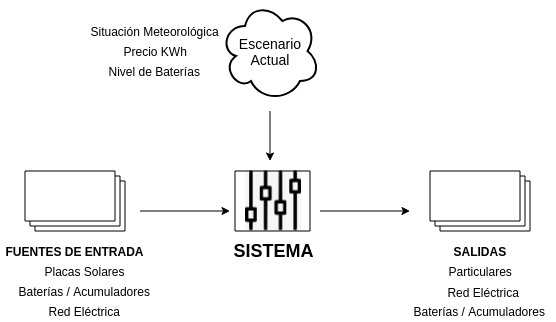
\includegraphics[width=8cm]{figs/Abstract.png}
	\caption{Dibujo del sistema}
\end{figure}


\chapter{Objetivos}
\label{cap:Objetivo}
A continuación se expone el objetivo de este trabajo así como una serie de objetivos parciales que se pretenden alcanzar durante el desarrollo de este \gls{TFG}.
\section{Objetivo Principal}
El objetivo principal de este \gls{TFG} es la construcción de un sistema para la simulación de la \textbf{distribución óptima} de energía entre \textbf{elementos generadores} y \textbf{elementos consumidores} en el hogar. Las fuentes de suministro de energía (elementos generadores) consideradas son:
\begin{itemize}
	\item Módulos fotovoltaicos.
	\item Red eléctrica.
	\item Baterías de almacenaje.
\end{itemize}
Como fuentes de consumo (elementos consumidores) se tendrán en cuenta:
\begin{itemize}
	\item Consumo energético del hogar.
	\item Consumo propio del sistema que se propone.
	\item Carga de baterías de almacenaje.
	\item Venta al mercado eléctrico como particular.
\end{itemize}
En la Figura~\ref{fig:schema} se muestra un esquema del sistema para facilitar su compresión: El sistema debe ser capaz de simular el flujo de energía entre las fuentes de entrada (\gls{EF}, \gls{ER} y \gls{EB}) y las salidas (\gls{CR}, \gls{CB}, consumo del hogar (C) y consumo propio del sistema ($ C_{int} $)). Esto se hará de manera óptima con el objetivo de minimizar el gasto económico dedicado en el hogar.

\begin{figure}[H]
	\centering
	\includegraphics[width=10cm]{figs/System.jpg}
	\caption{Esquema del sistema}
        \label{fig:schema}
\end{figure}

\section{Objetivos Parciales}
A lo largo del trabajo habrá que satisfacer una serie de subobjetivos.
\begin{enumerate}
	\item \textbf{Identificación y adquisición de los datos y variables que definen el sistema:}
	Estudio de las entradas y salidas del sistema y el grado de importancia que tiene cada una en cada situación. La información meteorológica será obtenida utilizando una \gls{API} oficial de \gls{AEMET}~\cite{Aemet}, y los datos del mercado eléctrico serán obtenidos utilizando la \gls{API} oficial e-sios de \gls{REE}~\cite{Ree}.

	\item \textbf{Establecer las relaciones entre las variables y restricciones que determinan el sistema:}
	Las variables obtenidas en el objetivo anterior estarán sujetas a unas restricciones que siempre vienen determinadas por la configuración de la instalación y por las propias propiedades físicas de generación y consumo de la energía, así como de las condiciones climáticas.

	\item \textbf{Implementar la generación optimizada de energía teniendo en cuenta las relaciones y restricciones existentes:}
	Una vez obtenidas las variables y restricciones que determinan el problema y conociendo su grado de implicación, se implementará la generación optimizada de energía en el sistema empleando algoritmos de optimización. Esto permitirá realizar simulaciones de optimización energética en un hogar y día determinados. Estas simulaciones darán como resultado la distribución energética que debería tener ese día para permitir el máximo aprovechamiento de la energía lo que redundaría en un coste económico mínimo para el hogar.

      \item \textbf{Hacer usable el sistema para realizar simulaciones a demanda:}
        Una vez se disponga de la funcionalidad de realizar simulaciones de optimización energética, se creará una aplicación web que permitirá interactuar a los usuarios con el sistema, configurando las características de su hogar y pudiendo realizar simulaciones de un día concreto. Gracias a los resultados de estas simulaciones, los usuarios podrán comparar la distribución energética y gasto económico que se hubiera producido empleando el sistema propuesto frente a lo ocurrido realmente con el consumo exclusivo de la red eléctrica.

      \item \textbf{Integración del sistema en la nube:}
        Cuando se cuente con una aplicación funcional, deberá integrarse en la nube para no tener dependencia de una máquina concreta haciendo honor a la tendencía cada vez más extendida del \textit{cloud computing}.

\end{enumerate}

\chapter{Antecedentes}
\label{cap:Antecedentes}
En este capítulo se exponen los conceptos de ciencias de la computación más importantes relacionados con este trabajo y el estado del arte actual.\\

\section{Sistema Inteligente}
Un agente inteligente es aquel que emprende la mejor acción posible ante una situación dada. El campo de la inteligencia artificial~\cite{Russ06} se centra en construir sistemas inteligentes que piensan como humanos, actúan como humanos, piensan racionalmente y actúan racionalmente. Como se puede observar, los cuatro enfoques están divididos en dos grupos: el primero se centra en los humanos y el segundo en la racionalidad. Un agente es racional si hace lo correcto en base a su conocimiento.El enfoque humano debe ser una ciencia empírica mientras que el enfoque racional se basa en una combinación de matemáticas e ingeniería. Estos cuatro enfoques de la inteligencia artificial han coexistido a lo largo de la historia.\\
\begin{itemize}
\item{El enfoque de la prueba de Turing (Actuar como humanos)}\\

  La prueba de Turing tenía como objetivo proporcionar una definición operacional y satisfactoria de inteligencia. Una máquina superaría la prueba si el examinador no fuese capaz de distinguir si el evaluado es una persona o un computador mediante una secuencia de preguntas. Para superarla un computador debe ser capaz de procesar el lenguaje natural, representar el conocimiento, contar con razonamiento automático y aprendizaje automático.
\item{El enfoque del modelo cognitivo (Pensar como humanos)}\\

Para determinar si una máquina es capaz de pensar de forma similar a un humano primero debe conocerse un mecanismo para ver como piensan los humanos: la ciencia cognitiva, en cuyo campo interdisciplinar convergen modelos computacionales de inteligencia artificial y técnicas de psicología intentando comprender el funcionamiento de la mente humana.
\item{El enfoque de las \textit{leyes del pensamiento} (Pensar racionalmente)}\\

  El \textit{modus operandi} de la mente humana se rige por silogismos, que son esquemas de estructuras de argumentación mediante los que se llega a conclusiones correctas si se parte de premisas correctas.
\item{El enfoque del agente racional (Actuar racionalmente)}\\

  Un agente racional actúa intentando alcanzar el mejor resultado y, en caso de haber incertidumbre, el mejor resultado esperado.
\end{itemize}
La inteligencia artificial y por ende los sistemas inteligentes tienen aplicación en numerosos ámbitos:
\begin{itemize}
\item{Resolución de problemas}
\item{Teoría de juegos}
\item{Robótica y automatización}
\item{Procesamiento del lenguaje natural}
\end{itemize}

\section{Problema de Satisfacción de Restricciones}
La programación por restricciones es una metodología software que permite resolver problemas de gran complejidad, típicamente NP. Esta metodología ha generado mucha expectación en el área de la inteligencia artificial desde la década de los 60, ya que tiene un gran potencial para la resolución de problemas reales. La idea básica de la programación por restricciones permite declarar una serie de restricciones sobre el dominio del problema que atañe, para después dar con soluciones que satisfacen las anteriores restricciones de la forma más optima posible. Así, un problema de satisfacción de restricciones~\cite{Russ06} está caracterizado por:
\begin{itemize}
	\item Un conjunto de variables, donde cada variable toma variables en un dominio.
	\item Un conjunto de restricciones, que permite representar las posibles combinaciones de valores válidos de las variables.
	\item La solución al \gls{PSR} será la asignación de valores a las variables de forma que se satisfacen las restricciones y se alcanza el objetivo, representado típicamente como una función a optimizar.
\end{itemize}
Las restricciones se caracterizan por su \textbf{aridad}, que viene a ser el número de variables que involucra. Pudiendo ser unarias, si solo involucran una variable; binarias, si involucran dos variables; y n-arias, si involucran más de dos variables. Se deben tener en cuenta un tipo de restricción adicional, ya que están presentes en este trabajo, como son las \textbf{restricciones lineales}, tal y como se representa en la Ecuación~\ref{eq:rest_lineal}
\begin{equation}
  \label{eq:rest_lineal}
  \forall_{i} \in A :  a_{i}x_{i} (<,\leq,=,\geq,>,\neq) c
\end{equation}
siendo a el coeficiente de la variable x y c constante, y A el conjunto de valores desde i hasta n. Esto se traduce como n-i restricciones, pues una restricción lineal realmente es el conjunto de restricciones de ese tipo desde i hasta n.\\
\section{Programación Lineal}
La programación lineal~\cite{Loom64} tiene como objetivo optimizar una función lineal cuyas variables están sujetas a un conjunto de restricciones lineales.
Se trata de un campo de la matemática muy efectivo para la resolución de este tipo de problemas. Históricamente, el concepto de programación lineal debe su nombre a John Von Neumann (1947), uno de los matemáticos más importantes del siglo XX gracias a sus contribuciones en las ciencias de la computación; y a George Dantzig (1947), cuyo trabajo intentaba asignar 70 puestos de trabajo a 70 personas mediante programación lineal. Las permutaciones necesarias para la asignación óptima de dichos puestos era igual a factorial de 70 (70!), algo muy grande, pues el número de combinaciones de variables es exponencial. Curiosamente, mediante programación lineal el problema se resuelve de manera eficiente pues el número de combinaciones se reduce en su mayor parte. La programación lineal puede ser aplicable a numerosos problemas comunes tales como:
\begin{itemize}
\item Asignación de horarios a profesores en un centro educativo para obtener la mayor productividad a la par que comodidad para profesor y alumno.
\item Distribución de elementos en almacenes de tal modo que se reduzca el costo de almacenamiento teniendo en cuenta la capacidad limitada.
\item Distribución de bienes entre compradores y consumidores de tal modo que las ganancias del intermediario sean máximas.
\end{itemize}
Como se puede observar, el problema de este \gls{TFG} está muy relacionado con el último ejemplo, pues se distribuye cantidad de energía entre fuentes de entrada y fuentes de salida de manera óptima para garantizar un gasto mínimo de consumo energético.\\

Para un problema de programación lineal pueden existir varios casos en su resolución:
\begin{itemize}
\item Existe una solución óptima.
\item Existen varias soluciones óptimas.
\item No existe solución.
\item Existen infinitas soluciones.
\end{itemize}
La situación deseada es la primera, pero puede ocurrir alguno de los otro casos. Estas situaciones pueden resolverse convirtiendo las restricciones que son inecuaciones (desigualdades) en igualdades.\\

Existen varios métodos de programación lineal. El más utilizado es conocido como el \textbf{método Simplex}, que se basa en evaluar solo algunos puntos extremos mediante dos condiciones:
\begin{itemize}
\item \textbf{Optimalidad}. La solución inferior relativa al punto de solución actual no se tiene en cuenta.
  \item \textbf{Factibilidad}. Una vez se encuentra una solución básica factible, sólo apareceran soluciones factibles.
\end{itemize}
Otro método de programación lineal es el método de ramificación y acotamiento \textit{branch and bound}, el cuál divide el problema en varios subproblemas de programación lineal, acotamiento que permite obtener soluciones óptimas que se mejora por cada subproblema.\\

\section{Estado del Arte}
Tal y como se ha comentado en el Capítulo~\ref{cap:Introduccion}, existe una gran demanda energética que desemboca en un encarecimiento de la energía eléctrica cada vez mayor. Esto hace que sea una problemática en la que se ha trabajado tanto en el ámbito comercial como en la investigación.\\

En el ámbito de la investigación se han encontrado varios estudios relacionados. Uno de ellos es una tesis doctoral perteneciente a la Universidad de Alicante: Modelado y simulación de la distribución de energía eléctrica en sistemas genéricos consistentes en diversas fuentes y múltiples modos de transmisión~\cite{Valdi13}. El trabajo de investigación de esta tesis doctoral aborda el problema de la distribución eléctrica en sistemas genéricos con varias fuentes de energía (eólica, hidroeléctrica, solar, etc). En este caso el sistema se implementa como un sistema multiagente en el que existen, cooperan y se comunican agentes que representan las fuentes energéticas, los consumos y los servicios. En la Figura~\ref{fig:tesis} se muestra la interfaz de usuario de este sistema, donde mediante unos parámetros de configuración se realiza la distribución de energía entre cada uno de los agentes involucrados.\\
\begin{figure}[H]
	\centering
	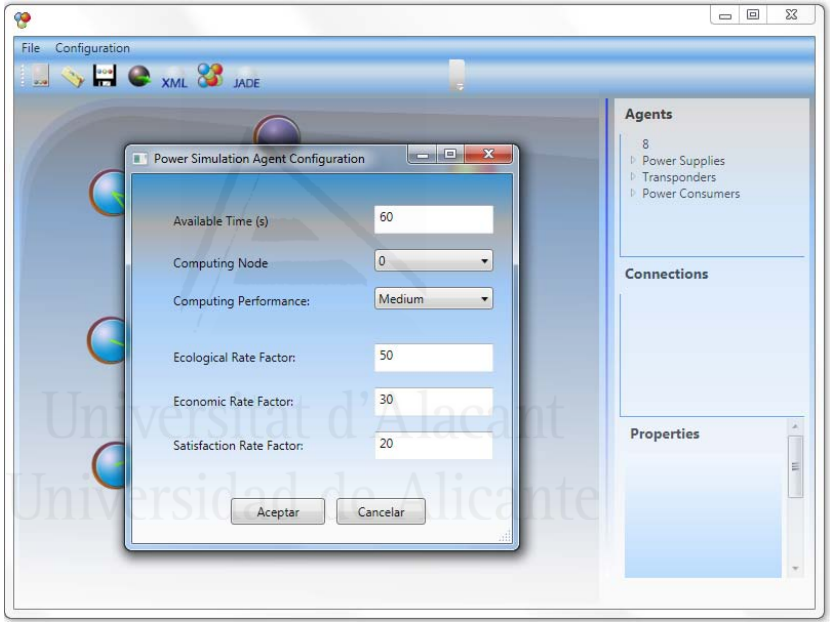
\includegraphics[width=10cm]{figs/tesis.png}
	\caption{Formulario de optimización de la aplicación perteneciente a la tesis doctoral de la Universidad de Alicante}
        \label{fig:tesis}
\end{figure}

En el ámbito comercial, existen varias aplicaciones móviles y web relacionadas con esta temática. A continuación se exponen algunas de ellas:
\begin{itemize}
  \item \textbf{Mi.Luz:} Se trata de una aplicación móvil disponible para iOS y Android que permite conocer el precio del KWh en cada momento del día, para que así el usuario establezca el consumo eléctrico en su hogar en las horas más baratas (Figura~\ref{fig:miluz}).
    \begin{figure}[!h]
	\centering
	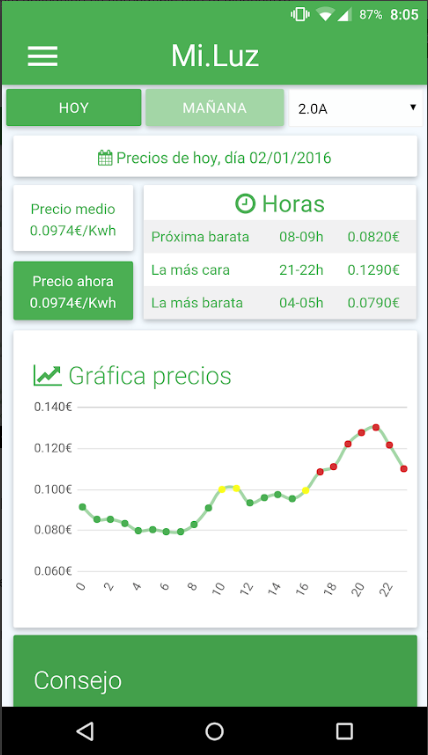
\includegraphics[width=4cm]{figs/miluz.png}
	\caption{Dashboard de la aplicación Mi.Luz}
        \label{fig:miluz}
\end{figure}
\item \textbf{Área Personal - Endesa:} Endesa brinda a sus clientes un área personal donde permite consultar el consumo realizado en un día determinado en su hogar, desglosado en horas. Además permite la descarga de ficheros con el consumo del hogar. Esta funcionalidad será de utilidad en este \gls{TFG}.
\item \textbf{Virtual Energy Advisor:} Aplicación ganadora del premio \textit{Barcelona Smart City App Hack}. Mediante la introducción de facturas del hogar y perfil, la aplicación ofrece información adaptada en tiempo real, previsiones de consumo y alertas en las horas de menor precio.
\item \textbf{Mirubee:} Es una aplicación móvil disponible para iOS y Android. Mediante la instalación de un medidor inteligente en el cuadro eléctrico del hogar, la aplicación analiza el patrón de consumo que se produce y a partir de ello proporciona indicaciones personalizadas para ahorrar en la factura de la luz. Mirubee fue creado por una \textit{start-up} española en 2011 con el objetivo de facilitar la monitorización de energía en las casas mediante una plataforma de prestaciones profesionales (Figura~\ref{fig:mirubee}).
  \begin{figure}[!h]
	\centering
	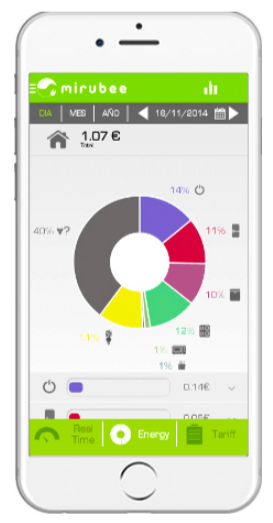
\includegraphics[width=4cm]{figs/mirubee.png}
	\caption{Informe de consumo del hogar en Mirubee}
        \label{fig:mirubee}
\end{figure}
\end{itemize}

\chapter{Metodología de trabajo}
\label{cap:Metodologia}
\section{Extreme Programming}
En el proyecto se emplea como metodología software un modelo iterativo e incremental,
que da lugar a una toma de decisiones a corto plazo lo que se traduce en ampliar requisitos y
soluciones en cada iteración (sprint) en función de las necesidades. Esto proporciona inmediatez
y funcionalidad en el proyecto lo que hace que exista una mayor motivación e implicación en
el mismo. Además, permite encontrar y solucionar errores a lo largo del trabajo y hace que el
cliente esté mas implicado debido a las numerosas entregas a lo largo del desarrollo del trabajo.

Como metodología de desarrollo y gestión de proyecto se usará \textbf{Extreme Programming (XP)}.\\
La programación extrema~\cite{Newk02} es un método ligero de desarrollo iterativo e incremental formulado por Kent Beck. Consta de varios períodos:
\begin{description}
	\item  \textbf{Exploración:}
	Período donde el objetivo será identificar, priorizar y estimar los requisitos del trabajo, por lo tanto se obtendrá como salida un documento de especificación de requisitos. El cliente expone sus necesidades y los programadores deben eliminar la ambigüedad para asegurarse de que los objetivos pueden ser alcanzados.

	\item \textbf{Punto de Fijación:}
	Se trata de una prueba rápida para profundizar en un determinado aspecto. Este punto se puede concretar durante la exploración o en cualquier otro momento en el que el equipo necesite resolver una cuestión.

	\item \textbf{Planificación de la Versión:}
	Cada versión del sistema proporciona un valor de negocio al cliente, quien, en cada planificación de versión, selecciona las historias o requisitos que van a ser implementados. Esto proporciona el máximo valor de negocio aunque no sea lo más acertado técnicamente.

	\item \textbf{Planificación de la Iteración:}
	Cada versión se divide en varias iteraciones. La longitud de iteración del trabajo se decide al principio y se mantiene constante durante el desarrollo. El equipo proporciona al cliente una estimación que representa cuanto trabajo se puede hacer en la iteración y el cliente selecciona que es lo que se implementará durante la iteración. Por lo tanto, se mantiene el marco de trabajo anteriormente mencionado en la planificación de la versión.

	\item \textbf{Desarrollo:}
	El software se desarrolla para un caso de prueba. Cuando éste consigue satisfacerse se pasa al siguiente caso de prueba. Para integrar el código en el sistema principal se deben satisfacer todas las pruebas. Durante el desarrollo el equipo no debe intentar anticiparse a tareas futuras, solo centrarse en la tarea actual.

\end{description}

\section{Medios a utilizar}
\subsection{Medios Hardware}
\subsection{Medios Software}

\chapter{Resultados}
\label{cap:Resultados}
En este capítulo se explican los resultados obtenidos en cada uno de los sprints del desarrollo del trabajo y cómo se relacionan con los objetivos definidos.


[... Hablar acerca de los sprints, que se va a hacer ...]
\section{Identificación y adquisición de las variables del sistema}
En el primer sprint se busca identificar cada una de las variables que entran en juego en el sistema, así como su proceso de obtención.. Se debe tener clara la diferencia entre variables de entrada y salida y variables de control.
\subsection{Variables de entrada}
Son las fuentes de suministro de energía al sistema. Habrá un total de tres:
\begin{itemize}
	\item \textbf{Energía fotovoltaica (EF)}\\ Energía procedente de las placas solares. Su valor viene determinado por varios factores, como son el número de módulos fotovoltaicos instalados y la máxima potencia posible en cada momento, \textit{current module power} (CMP). Hace referencia a la potencia de salida, en watios que produce un panel fotovoltaico en condiciones de máxima iluminación solar, con una radiación de aproximadamente 1 kW/m2. Será dependiente de la situación meteorológica del momento, de cuya obtención se hablará mas adelante. Como se puede observar, tendrá un valor máximo de obtención, que representa el tope de energía que podemos obtener de los módulos fotovoltaicos en ese momento.
	\item \textbf{Energía de red (ER)}\\ Energía procedente de la compañía eléctrica como cliente particular. Al contrario que en el caso anterior, no existe un límite superior a la hora de obtener energía de esta fuente.
	\item \textbf{Energía almacenada en batería (EB)}\\ Energía obtenida de la batería de almacenaje, que se ha guardado previamente para su posterior uso cuando el resto de fuentes de entrada tengan un mayor costo. Al igual que la energía fotovoltaica tiene un límite superior y viene determinado por la cantidad de carga de la misma y la profundidad de descarga que se le puede realizar sin resultar perjudicial para su ciclo de vida, que debe ser de un 50\% como máximo.
\end{itemize}

Cómo se ha mencionado, la energía fotovoltaica en una hora t será dependiente de la situación meteorológica de esa hora, algo evidente.\\Para obtener dicha información se utiliza la API oficial de AEMET \cite{Aemet}. Una API (\textit{Application Programming Interface}) es un conjunto de reglas o especificaciones que permite a las aplicaciones proporcionar servicios a otras o comunicarse. Para su uso, se ha debido solicitar un \textbf{API key} ya que es una API cerrada, esto es, su uso está restringido a un conjunto cerrado de clientes. Para realizar una petición a la misma, debe incluirse el \textit{API key} mencionado anteriormente en la url solicitada, así como una serie de parámetros como el código del municipio que se desea consultar. La respuesta a la petición contiene la previsión meteorológica de las próximas 24 horas en ese municipio.\\Para esta funcionalidad se ha creado el módulo \textit{api\_aemet}, que contiene la función \textit{get\_weather}, la cual se muestra en el listado~\ref{lst:aemet}
\begin{lstlisting}[language=Python,float=ht,caption={Función para obtener los valores meteorológicos},label={lst:aemet}]
def get_weather (city):
    weather_buffer = []
    url = const.AEMET_URL.replace('$CITY', city)
    response = requests.get(url)
    data = response.json()

    if data['estado'] == 200:
        url = data['datos']
        response = requests.get(url)
        data = response.json()[0]
        weather_buffer = create_weather_buffer(data)
        return weather_buffer
    return None
\end{lstlisting}
 Nótese que la url para la petición es obtenida como una constante de \textit{const}, alias que hace referencia al módulo de constantes del proyecto: \textit{project\_constants}. Este método realiza una petición a la API mediante la librería \textit{requests}~\cite{Kenn11}, y en caso de obtener un código de éxito (código de estado http 200), procesa la respuesta en la función \textbf{create\_weather\_buffer} y devuelve una lista con los 24 estados meteorológicos, correspondientes a las 24 horas de la simulación, del tipo: ["Despejado", "Poco Nuboso", "Despejado", ..., "Despejado"]\\

Las variables de entrada no son excluyentes, es decir, se puede obtener un tanto por ciento de la energía requerida procedente de cada una de ellas, lo que vendrá determinado por el precio en ese momento de cada una, ya que lo que buscamos es minimizar el gasto producido. A continuación se muestra el modo de determinación de los precios de las variables de entrada en una hora t: \\

	El precio de la energía fotovoltaica se calcula a partir de la inversión realizada en la instalación de los módulos fotovoltaicos y la cantidad de años en los que se desea amortizar dicha inversión. Así, el precio en €/Kw de EF se toma a partir de la fórmula~\ref{eq:costoEF}
	\begin{equation}
          \label{eq:costoEF}
	Costo_{EF} = \frac{coste_{anual}}{promedio^{kw}_{anual}} \textup{\euro}/kw
	\end{equation}
	Siendo el coste anual la cantidad invertida entre el número de años(n) en amortizarla, cómo se puede observar en la fórmula~\ref{eq:inversionEF}
	\begin{equation}
          \label{eq:inversionEF}
	Coste_{anual} = \frac{inversion}{n} \textup{\euro}
	\end{equation}


	El precio de la energía de red es el ya comentado PVPC. Para obtenerlo, se hace uso de la \textbf{API oficial de Red Eléctrica de España (e-sios)} \cite{Ree}. Para su uso se ha debido solicitar un \textit{Token} de acceso que se utiliza en las llamadas a la misma, al tratarse de una API cerrada análogamente al caso de la API de AEMET. Para el procesado de esta API se ha creado el módulo \textit{api\_esios}, que contiene la función \textit{get\_incoming\_prices}, la cuál se muestra en el listado~\ref{lst:esios}

	\begin{lstlisting}[language=Python,float=ht,caption={Función para obtener los valores del precio eléctrico},label={lst:esios}]
	def get_incoming_prices(indicator, start, end):
	   url = const.ESIOS_URL.replace('$INDICATOR', indicator)
	   url = url.replace('$START_DATE', dt.datetime.strftime(start, '%Y/%m/%d'))
	   url = url.replace('$END_DATE', dt.datetime.strftime(end, '%Y/%m/%d'))

	   response = requests.get(url, headers=HEADERS)
	   if response.status_code == 200:
	      data = response.json()
	      price_buffer = create_price_buffer(data, start)
	      return price_buffer
	   return None
	\end{lstlisting}

	Esta función es llamada desde el proyecto con el indicador deseado, que se corresponde con el precio que se desea consultar (en este caso PVPC), cuyo código numérico es obtenido de las constantes del proyecto, al igual que la url necesaria para la petición (ESIOS\_URL), que se forma con los parámetros adecuados y se realiza la petición \textit{get} haciendo uso de la librería \textit{requests}~\cite{Kenn11}. En este caso el \textit{API key} no se concatena en la url, si no que debe incluirse en la cabecera de la petición en un campo específico, ya que se trata de una autenticación por token como tal. Si la petición ha sido exitosa (código de respuesta http 200), la función retornará un \textit{buffer} de tamaño 24, que se corresponde con los valores del PVPC en las 24 horas definidas en la simulación. Para ello llama a \textit{create\_price\_buffer}, que se encargará de generar la lista con los 24 valores del precio solicitado procesando la respuesta recibida de la petición a la API.
	De esta manera se consigue el precio por Kw de la energía de red en cada momento.

	Por último, el precio de la energía de baterías se puede calcular de un modo muy parecido al de la energía fotovoltaica. Hace referencia al coste que supone extraer energía almacenada en la batería y está relacionado con la inversión realizada en la batería~\ref{eq:costoEB}
	\begin{equation}
          \label{eq:costoEB}
	Costo_{EB} = \frac{coste_{anual}}{capacidad_{bat}\cdot182,5} \textup{\euro}/kw
	\end{equation}
	Habiendo obtenido previamente el coste anual de forma similar a la fórmula~\ref{eq:inversionEF}. La constante 182,5 hace referencia al número de días del año (365) multiplicado por 0.5, debido a que no se va a realizar una profundidad de descarga mayor al 50\% de la capacidad total de la batería. El valor obtenido es el precio que supone recoger 1 Kw de la batería.
\subsection{Variables de salida}
Representan las fuentes de consumo de energía del sistema. Habrá un total de cuatro:
\begin{itemize}
\item \textbf{Consumo del hogar (C)}\\Demanda energética del hogar en cuestión, cuantía que debe ser satisfecha siempre, ya que es la energía que necesita el hogar para su uso cotidiano. En este trabajo fin de grado se ha decidido trabajar con clientes de la empresa eléctrica Endesa S.A., pues el hogar del alumno es su cliente lo que permitirá trabajar con información real. Además cuenta con un área privada de cliente que permite acceder a datos analíticos del hogar (Figura~\ref{fig:endesa}) y permite descargar ficheros en formato de texto con el consumo por horas de un día determinado en el hogar del cliente, justo lo que se necesita para dotar de valor esta variable. Para adaptar la información del fichero al valor de la variable se ha creado la función \textit{read\_from\_file(filename)} del módulo \textit{client\_consumption} que devuelve una lista con los 24 consumos de las 24 horas de la simulación en Kilowatios, obtenidos del fichero proporcionado.
  \begin{figure}[!h]
    \centering
    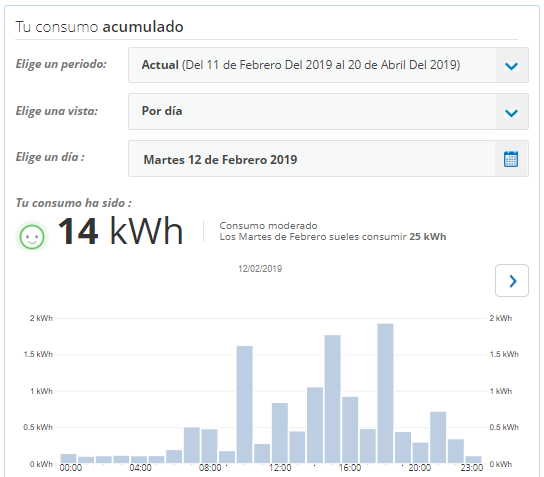
\includegraphics[width=10cm]{figs/Endesa.PNG}
    \caption{Panel de control del área cliente Endesa}
    \label{fig:endesa}
  \end{figure}
\item \textbf{Consumo interno del sistema ($ C_{int} $)}\\El sistema propuesto tiene un consumo constante de funcionamiento, cuyo valor se ha estimado en aproximadamente 2 Kw al día, alrededor de unos 0,088 watios por hora. Consta del consumo por funcionamiento de placas fotovoltaicas y realización de carga y descarga de batería.
	\item \textbf{Carga de batería (CB)}\\Cantidad de energía que se almacena en la batería para su posterior uso (almacenaje en batería). Esta variable cobra sentido en el caso de un abaratamiento de alguna fuente de generación de energía, lo que propicia que se obtenga más de la necesitada y se almacene para cuando el precio sea mayor.
	\item \textbf{Vertido al mercado eléctrico (CR)}\\Cantidad de energía que se vende al mercado eléctrico. Como particular, se puede disponer de una instalación fotovoltaica y verter energía a la red eléctrica, aunque es una práctica sujeta a numerosas trabas legales y dificultades en las que no se entrará en el desarrollo de este trabajo fin de grado. Esta energía se vertería al intramercado de red conocido como el mercado SPOT, aquel donde los activos que se compran o venden se entregan al precio de mercado del momento de la compra/venta.
\end{itemize}

Como se puede observar, el vertido al mercado eléctrico es un consumo que tiene un beneficio económico que ha de tenerse en cuenta. Existe una retribución por Kw vertido a la red dependiente del momento del día, ya que como se ha comentado antes, el valor de compra/venta del mercado SPOT varía. Para la obtención de estos valores se vuelve a hacer uso de la ya mencionada API e-sios, proporcionando a la función \textit{get\_incoming\_prices} el indicador del precio SPOT, presente en el fichero de constantes del proyecto. Análogo a la obtención del PVPC, se retorna un buffer con los 24 valores requeridos del precio SPOT correspondientes a las 24 horas a simular.\\

Aunque a priori parezca que el hecho de cargar las baterías no tiene una compensación económica, esto no es del todo correcto. Existe un beneficio económico, aunque no directo, con esta práctica. Puede ser explicado como la cantidad ahorrada por almacenar esa energía y no consumirla, ya que se ha pagado por ella. Este valor puede verse como el mínimo de los precios de las fuentes de generación de energía en el momento de la carga. Veamos un breve ejemplo:\\En la hora t se ha obtenido energía fotovoltaica a un precio de 0,11 € el Kwh. Por otro lado, se ha obtenido energía de la compañía eléctrica contratada a un precio de 0,14 € el Kwh. El beneficio económico indirecto por cargar un Kw de energía en batería en esta hora t será de 0,11 €.

\subsection{Variables de control}
Los valores de las variables definidas anteriormente son los que se intentan optimizar, pero existe otro conjunto de variables conocido como las variables de control. Aunque se denotan como variables, en el caso concreto de una simulación son constantes, ya que sus valores están predefinidos para la simulación del modelo. Este conjunto está formado por los valores de los que dependen las variables de entrada y salida y en función de los que se busca una optimización, y caracterizan tanto la simulación como la situación en una hora determinada.\\
Este conjunto está formado por:
\begin{itemize}
	\item \textbf{Fecha de inicio}\\ Valor que hace referencia al inicio de la simulación. Este valor es representado mediante el módulo datetime de Python. Datetime~\cite{Dtpy} es un módulo de la librería estándar de Python que permite manipular y trabajar con fechas. Este valor será un día y una hora de ese día.
	\item \textbf{Fecha de fin}\\ Corresponde al fin de la simulación. Siempre será 24 horas a partir de la fecha de inicio. Al igual que el anterior, se representa haciendo uso de datetime.
	\item \textbf{Número de módulos fotovoltaicos}\\ El número de módulos fotovoltaicos juega un papel fundamental. A mayor número de módulos, se producirá mas energía, pero mayor deberá ser la inversión para adquirirlos.
	\item \textbf{Precio de un módulo fotovoltaico}\\ En este trabajo el tipo de módulo fotovoltaico sera el se suele usar a nivel particular, de tamaño pequeño, con una potencia nominal en condiciones ideales de 50 watios hora~\ref{fig:pv_module}. Este modulo tiene un precio por unidad de 40 €, por lo tanto este valor tendrá el mismo valor en todas las simulaciones.
          \begin{figure}[!h]
            \centering
            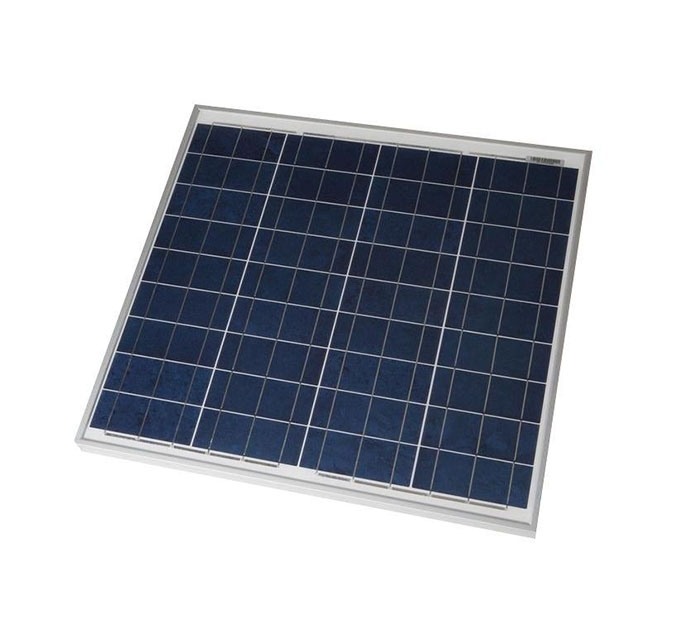
\includegraphics[width=6cm]{figs/panel_solar.jpg}
            \caption{Panel fotovoltaico de 50 W}
            \label{fig:pv_module}
          \end{figure}
	\item \textbf{Años en amortizar la inversión de los módulos fotovoltaicos}\\ El número de años en los que se desea amortizar la inversión realizada en la adquisición de los módulos fotovoltaicos, exclusivamente mediante su uso. Como se ha comentado anteriormente, no es algo trivial ya que determinará en gran medida el precio de extracción de energía fotovoltaica.
	\item \textbf{Precio de la batería}\\ En este trabajo el tipo de batería usado será una batería estacionaria~\ref{fig:bateria} compuesta por plomo abierto y gel. Este tipo de batería esta compuesta por dos vasos de 2V cada uno que disponen de un amplio rango de autonomía y una vida útil bastante larga, alrededor de unos 20 años. Son aconsejadas en instalaciones con un consumo medio (microondas, horno, lavadora, aire acondicionado, etc), es decir, perfectas para un hogar de tamaño normal. Cómo su tensión es de 2V, se debe instalar un total de 6 vasos en serie, al estar la instalación solar a 12V. Su precio es elevado debido a la gran capacidad, siendo un precio de 7900 € el de la obtención de los 6 vasos.
           \begin{figure}[!h]
            \centering
            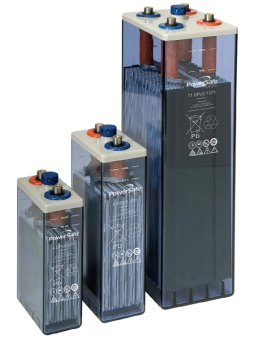
\includegraphics[width=4cm]{figs/bateria.jpg}
            \caption{Batería estacionaria}
            \label{fig:bateria}
          \end{figure}
	\item \textbf{Capacidad de la batería}\\ El tipo de batería usado, es decir, batería estacionaria de 6 vasos, tiene una capacidad total de aproximadamente 21 Kw. La profundidad de descarga de este tipo de batería es aproximadamente del 50\%, esto es, como se comento durante la explicación de las variables de entrada y salida, el tanto por ciento que se puede descargar dicha batería sin resultar perjudicial para su salud y por lo tanto afectar a su ciclo de vida útil.
	\item \textbf{Nivel de carga inicial de la batería}\\ Variable de control que define el estado inicial de la batería a la hora de realizar la simulación del modelo. Esto es la cantidad de energía que tiene almacenada la misma.
	\item \textbf{Años en amortizar la inversión de la batería}\\ Como ocurre en el caso de la inversión fotovoltaica, se debe determinar el número de años en los que se desea realizar la amortización de la inversión por adquirir la batería. Al tratarse de un valor mucho mas elevado debe ser mayor al del caso anterior, ya que si no se dispararía el precio de descargar las baterías y dejaría de ser una entrada a tener en cuenta al no resultar rentable.
\end{itemize}
Con esto quedan identificadas cada una de las variables que entran en juego en el modelo, así como su medio de adquisición.

\section{Aplicación de lógica difusa para la determinación de los estados meteorológicos}
En el segundo sprint se describe el procedimiento llevado a cabo para el uso de los estados meteorológicos obtenidos de la API de AEMET~\cite{Aemet}.

Tal y como se comentó en el sprint anterior, la respuesta a la petición \textit{requests} recibida por dicha API consta de estados meteorológicos en formato de cadena de texto. Un ejemplo de respuesta se muestra (simplificado) en el listado 4.3. (\textcopyright AEMET)

\begin{lstlisting}[numbers=none,caption={Ejemplo de respuesta de la API - AEMET}]]
{
 origen: {
	productor: "Agencia Estatal de Meteorología - AEMET. Gobierno de España",
	web: "http://www.aemet.es",
	language: "es",
	copyright: "AEMET. Autorizado el uso de la información y su reproducción citando a AEMET como autora de la misma.",
	notaLegal: "http://www.aemet.es/es/nota_legal"
 },
 elaborado: "2019-2-12",
 nombre: "Consuegra",
 provincia: "Toledo",
 prediccion: {
 	dia: [
		{
		 estadoCielo: [
					{
					 periodo: "08",
					 descripcion: "Cubierto"
					},
					{
					 periodo: "09",
					 descripcion: "Cubierto con lluvia escasa"
					},
					{
					 periodo: "10",
					 descripcion: "Cubierto con lluvia escasa"
					},
					{
					 periodo: "11",
					 descripcion: "Cubierto"
					},
					...
		 ]
		}
	}
}
\end{lstlisting}

Cómo se puede observar, en el campo 'predicción' existe un subcampo 'estadoCielo' (entre otros que se han obviado por no ser de interés en este trabajo) que contiene una lista con los estados meteorológicos. Cada elemento de la lista contiene dos valores: período (hora del día de esa previsión) y descripción (cadena de texto que describe el estado del cielo). Claramente existe un problema, ya que para la determinación de la máxima energía fotovoltaica posible en una hora determinada debe conocerse la potencia nominal posible (potencia que es capaz de suministrar el módulo fotovoltaico), directamente proporcional al estado meteorológico, el cuál es un texto que describe la situación y no un valor numérico que representa los watios que puede dar un módulo en esas condiciones, y a priori no se dispone de una forma directa de relacionarlas. \\

Se emplea \textbf{lógica difusa} para poder resolver la problemática mencionada anteriormente.
\subsection{Lógica difusa}
La teoría de la lógica difusa proporciona un marco matemático que permite modelar la incertidumbre de los procesos cognitivos humanos para poder ser tratable por un computador. Estos procesos cognitivos hacen referencia a expresiones del tipo:
\begin{itemize}
	\item Si no vives \textit{lejos} puedes ir en bicicleta. 
	\item Si hace \textit{mucho} frío llévate un chaquetón. 
\end{itemize} 
Los humanos son capaces de interpretar estos valores rápidamente, aunque no existe un valor cuantitativo que indique la distancia a la que se refiere la palabra \textit{lejos} o cuánto es \textit{mucho} frío. Sin embargo, las máquinas tienen algún que otro problema. Si se intentan trasladar estas reglar a código, aparecen dificultades ya que no se puede procesar numéricamente. Una opción es definir intervalos de valores que comprende cada palabra (por ejemplo, tomando \textit{lejos} como la distancia comprendida entre 5 y 10 kilómetros), pero esto no es preciso ya que para un computador, la distancia de 5,01 kilómetros sería lejos rotundamente, cuando en realidad la interpretación correcta no es así. Con ésto queda a la vista que la lógica convencional no trata de forma eficiente este problema. La solución pasa por emplear un método de razonamiento afín a la lógica difusa. \\

La lógica difusa permite representar matemáticamente la \textbf{incertidumbre}, mediante el empleo de herramientas formales. Según Zadeh~\cite{Zad73}, "\textit{Cuando aumenta la complejidad, los enunciados precisos pierden su significado y los enunciados útiles pierden precisión.}", es decir, \textit{los árboles no te dejan ver el bosque}, pues prácticamente cualquier problema del mundo puede resolverse partiendo de unas variables de entrada y buscando obtener como objetivo un conjunto de variables de salida. La lógica difusa establece esa relación entre variables de forma correcta.

\subsection{\textit{Fuzzy Sets}}



\begin{figure}[!h]
	\centering
	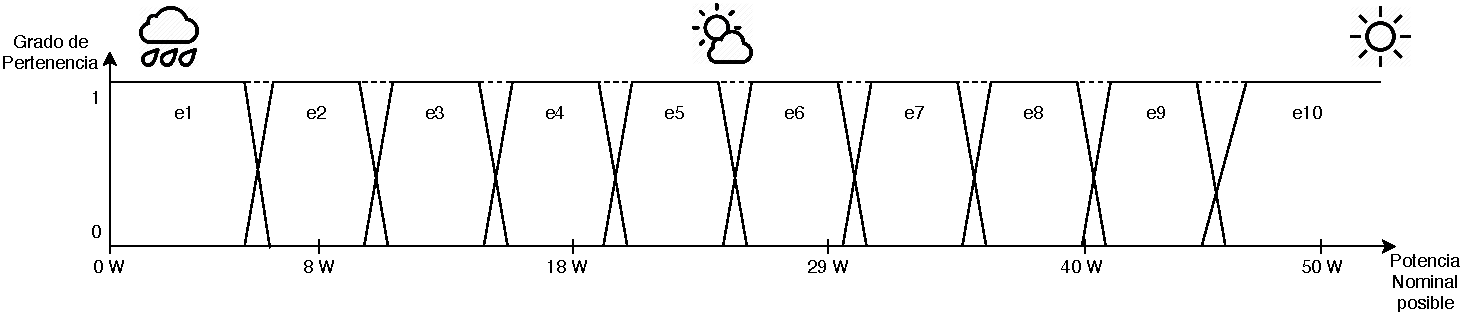
\includegraphics[width=17cm]{figs/Fuzzy_diagram.pdf}
	\caption{\textit{Fuzzy sets de los estados meteorológicos}}
\end{figure}
\section{Creación de las relaciones y restricciones propias del modelo}
Cómo se comento en el capítulo relativo al Objetivo del trabajo fin de grado, éste se aborda como un \textbf{problema de satisfacción de restricciones}.\\

La programación por restricciones es una metodología software que permite resolver problemas de gran complejidad, típicamente NP. Ésta metodología ha generado mucha espectación en el área de la inteligencia artificial desde la década de los 60, ya que tiene un gran potencial para la resolución de problemas reales. La idea básica de la programación por restricciones es primero declarar una serie de restricciones sobre el dominio del problema que atañe, para después dar con soluciones que satisfacen las anteriores restricciones de la forma más optima posible. Así, un problema de satisfacción de restricciones~\cite{Russ06} está caracterizado por:
\begin{itemize}
	\item Un conjunto de variables, donde cada variable dispone de un dominio de valores que puede tomar.
	\item Un conjunto de restricciones, que permite conocer las posibles combinaciones de las variables.
	\item La solución al PSR será la asignación de valores a las variables de forma que se satisfacen las restricciones y se alcanza el objetivo, representado típicamente como una función a optimizar.
\end{itemize}
Las restricciones se caracterizan por su \textbf{aridad}, que viene a ser el número de variables que involucra. Pudiendo ser unarias, si solo involucran una variable; binarias, si involucran dos variables; y n-arias, si involucran más de dos variables. Se deben tener en cuenta un tipo de restricción adicional, ya que están presentes en este trabajo, como son las \textbf{restricciones lineales}, expresadas teóricamente de la forma~\ref{eq:rest_lineal}
\begin{equation}
  \label{eq:rest_lineal}
  \sum_{i}^{n} a_{i}x_{i} (<,\leq,=,\geq,>,\neq) c
\end{equation}
siendo a el coeficiente de la variable x y c constante.\\

\subsection{Variables del PSR}

En los sprints 1 y 2 se identificaron las variables del problema, las cuáles están divididas en tres grupos: variables de entrada, variables de salida y variables de control. Sin embargo conviene mencionar cuáles de estas variables son las propias del problema de satisfacción de restricciones, y cuáles formarán las restricciones. El objetivo del problema es obtener valores de energía para los paneles fotovoltaicos, baterías y red eléctrica, de tal modo que se cubra la demanda energética del hogar y que el gasto económico sea el menor. Es por esto que las variables propias del problema de satisfacción de restricciones serán:
\begin{itemize}
\item \textbf{Energía fotovoltaica (EF)}. Energía obtenida de los módulos fotovoltaicos.~\ref{eq:dom_ef}
\begin{equation}
        \label{eq:dom_ef}
        Dom_{EF} = [0, EF_{max}]
\end{equation}
\item \textbf{Energía de red (ER)}. Energía importada de la red eléctrica.~\ref{eq:dom_er}
\begin{equation}
        \label{eq:dom_er}
        Dom_{ER} = [0, +\infty)
\end{equation}
\item \textbf{Energía de batería (EB)}. Energía obtenida de la batería.~\ref{eq:dom_eb}
\begin{equation}
        \label{eq:dom_eb}
        Dom_{EB} = [0, +\infty)
\end{equation}
\item \textbf{Consumo de batería (CB)}. Energía consumida para cargar la batería.~\ref{eq:dom_cb}
\begin{equation}
        \label{eq:dom_cb}
        Dom_{CB} = [0, +\infty)
\end{equation}
\item \textbf{Consumo de red (CR)}. Energía vertida a red a cambio de retribución económica.~\ref{eq:dom_cr}
\begin{equation}
        \label{eq:dom_cr}
        Dom_{CR} = [0, +\infty)
\end{equation}
\end{itemize}

Las restricciones estarán definidas en función de dichas variables y cada solución al problema estará formada por un valor para cada una de estas variables. Éstos valores satisfacen las restricciones y además serán los óptimos para que se produzca el menor gasto económico posible. El resto de variables (variables de control) determinarán las propias restricciones y el valor de las anteriores dependerá de éstas en una hora concreta t, entre 0 y 24h.\\

\subsection{Restricciones del PSR}
A continuación se determinan las restricciones a las que está sometido el modelo en una hora t:
\begin{itemize}
\item \textbf{Toda la energía generada debe ser consumida}.~\ref{eq:restr1}\\ \\Hace referencia al principio básico de la energía, la energía que se produce se consume de un modo u otro, no es posible que la suma de las variables correspondientes a la generación de energía (EB, ER y EF) sea distinta a la suma de las variables que hacen referencia al consumo de energía (CR, CB, $ C_{int} $ y C). Ésto debe producirse en cada una de las horas de la simulación. Así, tenemos una restricción lineal y n-aria correspondiente a la suma de las 24 horas correspondientes a una simulación, por lo que ésta restricciones a efectos prácticos es tomada como 24 restricciones a cumplir.
\begin{equation}
        \label{eq:restr1}
        \sum_{i=0}^{23} EF_{i}+ER_{i}+EB_{i} = CR_{i}+CB_{i}+C_{int}+C
\end{equation}

\item \textbf{No se puede producir energía fotovoltaica durante la noche}.~\ref{eq:restr2}\\ \\Algo obvio, pues sin luz solar la energía fotovoltaica no es posible. Ésto no está controlado en la API AEMET, ya que las peticiones relativas a la noche no reflejan una descripción propia del tiempo nocturo, si no que devuelve los mismos valores independientemente de si existe luz solar, por lo que debe manejarse mediante una restricción. Para este trabajo las horas de la noche serán las pertenecientes al intervalo temporal desde las 22:00 pm hasta las 7:00 am. Cómo posible trabajo futuro, podría determinarse este intervalo en función de la estación del año para que pueda ser un intervalo con mayor grado de efectividad. Se trata de una restricción unaria, donde para ciertos valores de t, EF debe ser 0. Es por esto que esta restricción a efectos prácticos es tomada como 9 restricciones (las 9 horas de noche definidas anteriormente)
\begin{equation}
        \label{eq:restr2}
        EF_{noche} = 0
\end{equation}

\item \textbf{La energía fotovoltaica generada no puede ser mayor que la máxima energía fotovoltaica en t}.~\ref{eq:restr3}\\ \\No se puede superar el umbral de generación de energía fotovoltaica establecido por la potencia nominal máxima de esa hora t, pues se estaría violando la capacidad real de producción de los módulos fotovoltaicos del sistema. Es una restricción lineal unaria, ya que la energía fotovoltaica máxima de cada hora t es constante, pues como se comentó anteriormente, sólo es dependiente del número de módulos fotovoltaicos y la situación meteorológica (obtenida de la API AEMET). A efectos prácticos, esta restricción es tomada como 24 restricciones a cumplir referentes a las 24 horas de la simulación.
\begin{equation}
        \label{eq:restr3}
        \sum_{i=0}^{23} EF_{i} \leq EF_{i}^{max}
\end{equation}

\item \textbf{La energía obtenida de la batería no puede ser mayor que el nivel de batería actual teniendo en cuenta la profundidad máxima de descarga}.~\ref{eq:restr4}\\ \\Básicamente no se puede obtener una cantidad de energía mayor a la posible en esa hora t, que vendrá determinada por la diferencia entre el  nivel de carga disponible al comienzo de esa hora y la capacidad máxima de la batería por la profundidad de descarga (50\%), para evitar daños en su ciclo de vida útil. Restricción unaria, pues solo involucra la variable EB, ya que el resto de elementos de la restricción son constantes en una hora t (nivel de carga actual, capacidad máxima de la batería y profundida de descarga). Al igual que las restricciones anteriores es lineal y a efectos prácticos representa 24 restricciones a cumplir.
\begin{equation}
        \label{eq:restr4}
        \sum_{i=0}^{23} EB_{i} \leq nivel_{i-1} - capacidad_{max} * profundidad_{descarga}
\end{equation}

\item \textbf{El consumo para cargar la batería no puede ser mayor que la capacidad de la misma menos el nivel restante después de t}.~\ref{eq:restr5}\\Parecido a la restricción anterior, en esta se modela el hecho de cargar la batería (CB) en cada hora t, el cuál está condicionado por la cantidad de batería restante para completar la carga (100\%), obtenido mediante la diferencia entre la capacidad máxima de la misma y lo consumido en la hora t (nivel de carga antes de comenzar la hora t menos la energía consumida de batería en t). Restricción binaria pues involucra tanto el consumo de batería (CB) como la energía de batería (EB), siendo la capacidad máxima de la batería y el nivel de carga en t constantes. Es tomado como 24 restricciones ya que debe cumplirse en cada una de las 24 horas de una simulación.
\begin{equation}
        \label{eq:restr5}
        \sum_{i=0}^{23} CB_{i} \leq capacidad_{max}- (nivel_{i-1} - EB_{i})
\end{equation}

\end{itemize}

Por lo tanto, a efectos prácticos, el PSR tiene 81 restricciones que satisfacer para determinar los valores de las variables.

\subsection{Función Objetivo}
Cómo se ha comentado antes, un problema de satisfacción de restricciones está determinado por un conjunto de variables y sus dominios, un conjuntos de restricciones de esas variables, y un objetivo. Por el momento se dispone de los dos primeros, por que en este apartado se procede a determinar el último, \textbf{la función objetivo}.\\

Un PSR que cuenta únicamente con variables y restricciones para esas variables podrá tener numerosas soluciones, representadas como una tupla con valores para cada variable. Añadiendo un objetivo al PSR se consigue unificar la solución, pues de todas esas soluciones, sólo una optimizará un objetivo concreto, y contendrá los valores óptimos de cada variable para ello.\\

Como se ha comentado a lo largo del desarrollo de este trabajo fin de grado, el objetivo del problema es \textbf{minimizar el gasto económico} producido mediante la optimización de energía en cada simulación de 24 horas, por lo tanto se buscarán valores de las variables que, además de satisfacer el conjunto de restricciones, sean óptimos para que el gasto económico sea mínimo. Éste gasto económico es dependiente del precio en la hora t de cada una de las energías que representan las variables. De estos precios se habló y se implementó la forma de obtenerlos en el sprint 1. Sus valores son constantes en cada hora t. Dicho esto, la función objetivo a minimizar está formada por el sumatorio de los gastos económico en cada hora t, por lo que representa el gasto económico de toda la simulación.~\ref{eq:funcionObjetivo}
\begin{equation}
\label{eq:funcionObjetivo}
f(x) = \sum_{i=0}^{23} EF_{i}P_{i}^{F} + ER_{i}P_{i}^{R_{PVPC}} + EB_{i}P_{i}^{B_{out}} - CB_{i}P_{i}^{B_{in}} - CR_{i}P_{i}^{R_{SPOT}}
\end{equation}
Siendo:
\begin{itemize}
\item $ EF_{i}P_{i}^{F} $: Gasto económico producido al generar energía fotovoltaica en la hora t.
\item $ ER_{i}P_{i}^{R_{PVPC}} $: Gasto económico producido al importar energía a la compañía eléctrica en la hora t.
\item $ EB_{i}P_{i}^{B_{out}} $: Gasto económico producido al descargar la batería en la hora t.
\item $ CB_{i}P_{i}^{B_{in}} $: Ganancia económica producida al cargar la batería en la hora t.
\item $ CR_{i}P_{i}^{R_{SPOT}} $: Ganancia económica producida al verter energía al mercado eléctrico en la hora t.
\end{itemize}

En cada simulación se buscará que el valor de $ f(x) $ sea el menor posible y la solución al PSR de esa simulación será los valores que deben tomar las variables para hacerlo posible.

\subsection{Implementación de la clase Simulation}
Vistos los apartados anteriores, es la hora de implementar una clase para representar el modelo de simulación, y poder crear objetos que representan una simulación concreta. Esta clase se llama \textbf{Simulation}~\ref{fig:simulation} y está disponible en el módulo simulation.\\

Los atributos de clase de Simulation serán las variables de control que tendrá cada objeto correspondiente a una simulación:
\begin{itemize}
        \item start: variable de control referente a fecha de inicio de la simulación. Es de tipo datetime.
        \item end: variable de control referente a fecha de fin de la simulación. Al igual que start, es una variable de formato fecha (datetime).
        \item ef\_price: variable de control referente al precio de generar energía fotovoltaica. Se trata de un número tipo float, pues tendrá el mismo valor en toda la simulación (se obtiene a partir de la inversión realizada)
        \item er\_price: variable de control referente a los precios que tendrá el PVPC en cada hora de la simulación. Es una lista de 24 elementos de tipo float.
        \item eb\_price: variable de control referente al precio de descargar la batería. Es un número de tipo float ya que será igual en las 24 horas de la simulación.
        \item cr\_price: variable de control referente a los precios SPOT en cada hora de la simulación, es decir, el precio del vertido de energía a la red eléctrica.
        \item cb\_price: variable de control referente a los precios de cargar la batería. Cómo es dependiente de los precios de energía fotovoltaica y de red de cada hora t, se trata de una lista con 24 valores.
        \item battery\_capacity: variable de control referente a la capacidad total de la batería. Variable de tipo float.
        \item battery\_level: variable de control que representa el nivel inicial de carga de la batería. Variable de tipo float.
        \item discharge\_depth: variable de control referente a la profundidad de descarga permitida en la batería. Variable de tipo float.
        \item max\_ef\_buffer: Más que una variable de control, representa los 24 valores máximos posible de energía fotovoltaica, obtenidos como se comentó anteriormente mediante la información de la API AEMET y el número de módulos fotovoltaicos, por ende, se trata de una lista de 24 valores.
        \item c\_int: referente a la variable de control del consumo interno del sistema. Variable de tipo float.
        \item c: referente al consumo del hogar, lista de los 24 valores con el consumo del hogar en las 24 horas de la simulación.

Las funciones de esta clase sirven para calcular algunos de los atributos anteriores. En la figura~\ref{fig:simulation} se muestra la clase UML de Simulation.
\end{itemize}

\begin{figure}[H]
        \centering
        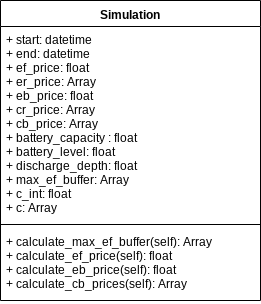
\includegraphics[width=6cm]{figs/simulation_class.png}
        \caption{Clase Simulation}
        \label{fig:simulation}
\end{figure}

En el próximo sprint se implementará cada una de las restricciones para permitir ejecutar la simulación.

\section{Generación optimizada de energía mediante programación lineal}
\section{Persistencia de datos y creación del servidor}

\chapter{Conclusiones}
\label{cap:Conclusiones}
En este capítulo se muestran las conclusiones obtenidas tras el desarrollo de este \gls{TFG} junto con posible desarrollo futuro a realizar que permitiría ampliar la funcionalidad del sistema.\\
\section{Satisfacción de objetivos}
El objetivo principal del \gls{TFG} ha sido la \textbf{construcción de un sistema inteligente para la simulación de la distribución óptima de energía entre elementos generadores y elementos cosumidores}. Dicho objetivo se ha completado satisfactoriamente durante el desarrollo. Se ha creado un sistema capaz de minimizar el coste energético de una instalación representada por un conjunto de variables, restricciones y condiciones climáticas en un día determinado.\\

El objetivo parcial referente a la \textbf{identificación y adquisición de los datos y variables que definen el sistema} se ha completado satisfactoriamente durante las iteraciones 1 y 2 del desarrollo (Secciones~\ref{sec:hito1} y~\ref{sec:hito2}), donde se trabajó en la obtención de las variables requeridas (precios de cada una de las energías, situación meteorológica, consumo, etc) y en su adaptación al sistema (transformación de los estados meteorológicos a valores discretos, tratado de cada una de las APIs utilizadas, etc).\\

Otro objetivo parcial era \textbf{establecer las relaciones entre las variables y restricciones que determinan el sistema}. Este objetivo se ha completado satisfactoriamente mediante el resultado obtenido de la iteración 3 (Sección~\ref{sec:hito3}) del desarrollo. En dicha iteración se trabajó en la definición del \gls{PSR} planteado, determinando los dominios de las variables que lo componen e identificando las restricciones relativas a la configuración de la instalación, propiedades físicas de generación y consumo de energía y condiciones climáticas. También se determina la función objetivo que dará solución al \gls{PSR} minimizando el coste energético.\\

El siguiente objetivo parcial pasaba por \textbf{implementar la generación optimizada de energía teniendo en cuenta las relaciones y restricciones existentes}. Hace referencia al núcleo del sistema, pues la satisfacción de este objetivo permitiría generar la optimización deseada. Este objetivo ha sido completado con éxito en la iteración 4 (Sección~\ref{sec:hito4}) haciendo uso de algoritmos de programación lineal que permiten minimizar la función objetivo generando una distribución óptima de energía.\\

El último objetivo parcial requerido era \textbf{hacer usable el sistema para realizar simulaciones a demanda}. La iteración 5 (\ref{sec:hito5}) del desarrollo consistió en la creación de una aplicación web que permitiera interactuar a los usuarios con el sistema, configurando las características de su hogar y pudiendo realizar simulaciones de un día concreto. Gracias a los resultados de estas simulaciones, los usuarios podrían comparar la distribución energética y gasto económico que se hubiera producido empleando el sistema propuesto frente a lo ocurrido realmente con el consumo exclusivo de la red eléctrica. Este objetivo se cumple con éxito pues se dispone de una aplicación totalmente funcional que cuenta con interfaz, lógica y persistencia encargada de realizar lo definido.\\

Finalmente, se definió un objetivo parcial para la \textbf{integración del sistema en la nube} obteniendo ubicuidad de acceso y desvinculación de la máquina local. Durante la iteración 6~\ref{sec:hito6} se realizó la migración a la nube, por un lado el servidor se integró en los servicios de Amazon Web Services (AWS) y por otro lado la base de datos fue integrada en los servicios ofrecidos por IBM Cloud. Esto demuestra que el objetivo se ha cumplido con éxito.\\
\section{Ámbito profesional}
En el ámbito profesional se han obtenido beneficios académicos al ampliar conocimientos acerca de sistemas inteligentes, uso de APIs de servicios, tecnologías de computación en la nube y algoritmos de optimización y desarrollo. Se han obtenido conocimientos en lo relativo a desarrollo de \textit{frontend}, marco donde el alumno no había trabajado anteriormente siendo necesario haber adquirido unas competencias con las que no se contaban antes de la realización de este trabajo.\\
Se ha estudiado y utilizado una metodología ágil de desarrollo software como es \textbf{programación extrema (XP)} que ha permitido al alumno obtener conocimientos acerca del uso de metodologías ágiles, elección de la más adecuada para un caso concreto y su aplicación, algo que será de verdadera utilidad y que constituye una base en su futuro profesional junto con los conocimientos adquiridos durante el grado. El haberse enfrentado al desarrollo de un proyecto software en un tiempo limitado, partiendo desde cero y dando como resultado un \textbf{sistema inteligente} usable, mantenible y mejorable ha permitido al alumno llevar a la práctica cada uno de los conceptos y habilidades obtenidas tras la realización del Grado en Ingeniería Informática.\\

Se ham ampliado y llevado a la práctica numerosos conocimientos en el software de control de versiones Git. El repositorio de este \gls{TFG} se ha estructurado en dos bloques: SOURCE y DOC, los cuáles contienen el software del sistema y la documentación del proyecto, respectivamente. Cada uno de ellos ha sido desarrollado paralelamente en dos ramas distintas y posteriormente mezcladas en la rama \textit{master}. En el caso del desarrollo, se ha creado una nueva rama partiendo de la propia \textit{source} por cada una de las iteraciones \gls{XP}, siendo mezcladas de nuevo en \textit{source} tras pasar la revisión del director. Para ello se han creado \textit{pull requests} por cada iteración, en cuyas descripciones se indicaban los puntos e historias de usuario desarrollados en la iteración, obtenidos del tablero Kanban de la misma.\\

Puesto que se han empleado herramientas de \textit{time tracking} típicas en el desarrollo ágil del software, se ha obtenido como resultado un total de 305 horas de trabajo imputadas. De esta cantidad de tiempo, un total de 169 horas corresponde a desarrollo software; 120 horas corresponden a documentación; y 16 horas han sido empleadas en reuniones de planificación, revisión y consulta de dudas con los directores.
\section{Trabajo futuro}
En cuanto al posible trabajo futuro se exponen a continuación mejoras que no se han podido implementar debido a la limitación de tiempo en la realización de un \gls{TFG}.
\begin{itemize}
\item \textbf{Alamacenar en base de datos las simulaciones realizadas}. El sistema realiza simulaciones cuyos resultados muestra y permite descargar al usuario, pero no se realiza una persistencia de los mismos por usuario. Resultaría interesante almacenar las simulaciones que realiza un usuario.
\item \textbf{Aplicar \textit{machine learning} a la base de datos para obtener conocimiento acerca del consumo eléctrico}. Mediante las simulaciones almacenadas comentadas anteriormente, se podrían aplicar algoritmos de aprendizaje automático a la base de datos cuando se cuente con un volumen representativo de datos pudiendo dar lugar a conocimiento.
\item \textbf{Aumentar la precisión de obtención de variables para generar resultados más concretos}. El valor de energía fotovoltaica es calculado en función del estado meteorológico actual y el número de módulos fotovoltaicos con los que se cuenta. Esto puede ser mucho mas preciso pues hay más factores dependientes como pueden ser el grado de incidencia de la luz solar en el módulo, viento, sensación térmica o desgaste de la placa que no se han podido tener en cuenta debido a la limitación temporal.
\item \textbf{Trabajar en la mejora y ampliación de la página web}. Puesto que el tiempo ha sido limitado han quedado pendientes posibles mejoras a realizar en la página web como son mayor control de sesiones, funcionalidad \textit{responsive} (adecuación al formato del dispositivo), con la que se cuenta de manera limitada pues algunos elementos se solapan si se accede desde determinados dispositivos móviles. Otra ampliación de la web si se implementa la persistencia de simulaciones sería añadir una nueva sección que permitiera consultar estadísticas y reportes de simulaciones realizadas por el usuario.
\item \textbf{Implementación de un bot que mediante \textit{web scraping} obtenga el consumo del usuario} en lugar de ser obtenido por medio de la carga de un fichero de texto por parte del cliente en la web. El usuario únicamente añadiría su cuenta de Endesa (con previa aceptación de permisos) y el bot se encargaría de obtener la información de su consumo para realizar simulaciones, teniendo únicamente que elegir el día de simulación.
\end{itemize}

% -------------------------




% -------------------------
%
% ANEXOS
%
% -------------------------
\appendix

% Tras este punto los capítulos se numeran con letras.
% Aquí todos los apéndices necesarios
\chapter{Reporte de Simulación 11/04/2019}
\label{cap:AnexoA}
\begin{lstlisting}[numbers=none,caption={Reporte de simulación 11/04},label={lst:simulationReport}]
-----------------------------------------------------
--------------- Simulacion Completada ---------------
-----------------------------------------------------
Inicio:	2019-03-11 00:00:00
Fin:	2019-03-12 00:00:00
Gasto: 0.6187091110614097 €

Valores a las 00:00 11/03/19
	- EF = 0.0 Kwh
	- ER = 0.19879999999999853 Kwh
	- EB = 0.0 Kwh
	- CR = 0.0 Kwh
	- CB = 0.0 Kwh
	- Consumo del Hogar = 0.11 Kwh
	- Consumo del Sistema = 0.0888 Kwh
----------------------------------------------
Valores a las 01:00 11/03/19
	- EF = 0.0 Kwh
	- ER = 0.16880000000000628 Kwh
	- EB = 0.0 Kwh
	- CR = 0.0 Kwh
	- CB = 5.329070518200751e-15 Kwh
	- Consumo del Hogar = 0.08 Kwh
	- Consumo del Sistema = 0.0888 Kwh
----------------------------------------------
Valores a las 02:00 11/03/19
	- EF = 0.0 Kwh
	- ER = 0.25479999999999947 Kwh
	- EB = 0.0 Kwh
	- CR = 0.0 Kwh
	- CB = 0.0 Kwh
	- Consumo del Hogar = 0.166 Kwh
	- Consumo del Sistema = 0.0888 Kwh
----------------------------------------------
Valores a las 03:00 11/03/19
	- EF = 0.0 Kwh
	- ER = 0.2297999999999938 Kwh
	- EB = 0.0 Kwh
	- CR = 0.0 Kwh
	- CB = 0.0 Kwh
	- Consumo del Hogar = 0.141 Kwh
	- Consumo del Sistema = 0.0888 Kwh
----------------------------------------------
Valores a las 04:00 11/03/19
	- EF = 0.0 Kwh
	- ER = 1.460599999999996 Kwh
	- EB = 0.0 Kwh
	- CR = 0.0 Kwh
	- CB = 1.2767999999999962 Kwh
	- Consumo del Hogar = 0.095 Kwh
	- Consumo del Sistema = 0.0888 Kwh
----------------------------------------------
Valores a las 05:00 11/03/19
	- EF = 0.0 Kwh
	- ER = 0.21480000000000388 Kwh
	- EB = 0.0 Kwh
	- CR = 0.0 Kwh
	- CB = 0.0 Kwh
	- Consumo del Hogar = 0.126 Kwh
	- Consumo del Sistema = 0.0888 Kwh
----------------------------------------------
Valores a las 06:00 11/03/19
	- EF = 0.0 Kwh
	- ER = 0.0 Kwh
	- EB = 0.27479999999999905 Kwh
	- CR = 0.0 Kwh
	- CB = 0.0 Kwh
	- Consumo del Hogar = 0.186 Kwh
	- Consumo del Sistema = 0.0888 Kwh
----------------------------------------------
Valores a las 07:00 11/03/19
	- EF = 0.0 Kwh
	- ER = 0.0 Kwh
	- EB = 0.3058000000000014 Kwh
	- CR = 0.0 Kwh
	- CB = 0.0 Kwh
	- Consumo del Hogar = 0.217 Kwh
	- Consumo del Sistema = 0.0888 Kwh
----------------------------------------------
Valores a las 08:00 11/03/19
	- EF = 0.816 Kwh
	- ER = 0.0 Kwh
	- EB = 0.0 Kwh
	- CR = 0.0 Kwh
	- CB = 0.15920000000000023 Kwh
	- Consumo del Hogar = 0.568 Kwh
	- Consumo del Sistema = 0.0888 Kwh
----------------------------------------------
Valores a las 09:00 11/03/19
	- EF = 0.266 Kwh
	- ER = 0.0 Kwh
	- EB = 0.5147999999999939 Kwh
	- CR = 0.0 Kwh
	- CB = 0.0 Kwh
	- Consumo del Hogar = 0.692 Kwh
	- Consumo del Sistema = 0.0888 Kwh
----------------------------------------------
Valores a las 10:00 11/03/19
	- EF = 0.266 Kwh
	- ER = 0.0 Kwh
	- EB = 0.10279999999999845 Kwh
	- CR = 0.0 Kwh
	- CB = 0.0 Kwh
	- Consumo del Hogar = 0.28 Kwh
	- Consumo del Sistema = 0.0888 Kwh
----------------------------------------------
Valores a las 11:00 11/03/19
	- EF = 1.816 Kwh
	- ER = 0.0 Kwh
	- EB = 0.0 Kwh
	- CR = 0.0 Kwh
	- CB = 1.511199999999997 Kwh
	- Consumo del Hogar = 0.216 Kwh
	- Consumo del Sistema = 0.0888 Kwh
----------------------------------------------
Valores a las 12:00 11/03/19
	- EF = 0.0 Kwh
	- ER = 0.0 Kwh
	- EB = 0.2378 Kwh
	- CR = 0.0 Kwh
	- CB = 0.0 Kwh
	- Consumo del Hogar = 0.149 Kwh
	- Consumo del Sistema = 0.0888 Kwh
----------------------------------------------
Valores a las 13:00 11/03/19
	- EF = 0.0 Kwh
	- ER = 0.0 Kwh
	- EB = 0.43680000000000163 Kwh
	- CR = 0.0 Kwh
	- CB = 0.0 Kwh
	- Consumo del Hogar = 0.348 Kwh
	- Consumo del Sistema = 0.0888 Kwh
----------------------------------------------
Valores a las 14:00 11/03/19
	- EF = 0.816 Kwh
	- ER = 0.0 Kwh
	- EB = 0.0 Kwh
	- CR = 0.0 Kwh
	- CB = 0.05020000000000202 Kwh
	- Consumo del Hogar = 0.677 Kwh
	- Consumo del Sistema = 0.0888 Kwh
----------------------------------------------
Valores a las 15:00 11/03/19
	- EF = 3.816 Kwh
	- ER = 0.0 Kwh
	- EB = 0.0 Kwh
	- CR = 0.0 Kwh
	- CB = 3.3882000000000057 Kwh
	- Consumo del Hogar = 0.339 Kwh
	- Consumo del Sistema = 0.0888 Kwh
----------------------------------------------
Valores a las 16:00 11/03/19
	- EF = 0.8160000000000001 Kwh
	- ER = 0.0 Kwh
	- EB = 0.0 Kwh
	- CR = 0.0 Kwh
	- CB = 0.3592000000000013 Kwh
	- Consumo del Hogar = 0.368 Kwh
	- Consumo del Sistema = 0.0888 Kwh
----------------------------------------------
Valores a las 17:00 11/03/19
	- EF = 0.816 Kwh
	- ER = 0.0 Kwh
	- EB = 0.0 Kwh
	- CR = 0.0 Kwh
	- CB = 0.5351999999999997 Kwh
	- Consumo del Hogar = 0.192 Kwh
	- Consumo del Sistema = 0.0888 Kwh
----------------------------------------------
Valores a las 18:00 11/03/19
	- EF = 0.0 Kwh
	- ER = 0.0 Kwh
	- EB = 0.2907999999999973 Kwh
	- CR = 0.0 Kwh
	- CB = 0.0 Kwh
	- Consumo del Hogar = 0.202 Kwh
	- Consumo del Sistema = 0.0888 Kwh
----------------------------------------------
Valores a las 19:00 11/03/19
	- EF = 0.8159999999999998 Kwh
	- ER = 0.0 Kwh
	- EB = 0.0 Kwh
	- CR = 0.14539999999999864 Kwh
	- CB = 0.4068000000000005 Kwh
	- Consumo del Hogar = 0.175 Kwh
	- Consumo del Sistema = 0.0888 Kwh
----------------------------------------------
Valores a las 20:00 11/03/19
	- EF = 0.266 Kwh
	- ER = 0.0 Kwh
	- EB = 5.116400000000001 Kwh
	- CR = 4.645600000000003 Kwh
	- CB = 0.0 Kwh
	- Consumo del Hogar = 0.648 Kwh
	- Consumo del Sistema = 0.0888 Kwh
----------------------------------------------
Valores a las 21:00 11/03/19
	- EF = 0.816 Kwh
	- ER = 0.0 Kwh
	- EB = 0.047999999999998266 Kwh
	- CR = 0.2962000000000007 Kwh
	- CB = 0.0 Kwh
	- Consumo del Hogar = 0.479 Kwh
	- Consumo del Sistema = 0.0888 Kwh
----------------------------------------------
Valores a las 22:00 11/03/19
	- EF = 0.0 Kwh
	- ER = 0.0 Kwh
	- EB = 0.4068000000000005 Kwh
	- CR = 0.0 Kwh
	- CB = 0.0 Kwh
	- Consumo del Hogar = 0.318 Kwh
	- Consumo del Sistema = 0.0888 Kwh
----------------------------------------------
Valores a las 23:00 11/03/19
	- EF = 0.0 Kwh
	- ER = 0.0 Kwh
	- EB = 0.3587999999999987 Kwh
	- CR = 0.0 Kwh
	- CB = 0.0 Kwh
	- Consumo del Hogar = 0.27 Kwh
	- Consumo del Sistema = 0.0888 Kwh
----------------------------------------------
\end{lstlisting}
 % Apéndice A (opcionales)
\chapter{Tests del proyecto}
\label{cap:AnexoB}
Las pruebas o \textit{tests} son la etapa del ciclo de vida del software que consiste en la implementación de casos de prueba unitarios sobre cada una de las funcionalidades de una aplicación. Completar los tests con éxito en una aplicación implica:
\begin{itemize}
\item La aplicación es utilizable.
\item Se logra obtener el resultado esperado o definido para cada funcionalidad de la aplicación.
\item Existe control y manejo de errores.
\item La ejecución se realiza en un tiempo aceptable.
\item Los requisitos definidos durante el diseño y desarrollo han sido implementados correctamente.
\end{itemize}

Se ha utilizado el framework \textbf{Nose} para implementación de casos de prueba en Python. Se implementan tests que comprueban cada uno de los módulos que componen el sistema. En el directorio \textbf{test} se encuentran todos los ficheros relativos a las pruebas. (Véase el \textit{tree} del listado~\ref{lst:testree})
\begin{lstlisting}[numbers=none,caption={Estructura del directorio \textit{test}},label={lst:testree}]
 --- test
    |-- factories
    |   |
    |    -- factory_models.py
    |-- tests_api.py
    |-- tests_app.py
    |-- tests_models.py
\end{lstlisting}

La factoría de modelos (\textit{factory\_models}) se encarga de generar un usuario o hogar a petición de los tests, lo que agiliza muchísimo el proceso y fomenta la reutilización de código.\\

Los tests de API se encargan de comprobar la funcionalidad de las APIs empleadas en el sistema (Esios y AEMET). Las peticiones son probadas ejecutando las funciones de cada módulo y comprobando si el resultado obtenido es un buffer de 24 posiciones en caso de probar el éxito, o un buffer vacío en caso de probar el fallo.

Los tests de modelos comprueban la corrección de cada uno de los modelos \textit{User} y \textit{Home} realizando inserciones correctas, erróneas, borrados, y demás operaciones en la base de datos de test. Para ello se configura la aplicación en modo test mediante el fichero de configuración \textit{test\_config}.

El módulo de test \textit{tests\_app} tiene una gran importancia, pues contiene los casos de prueba unitarios referentes al \textit{routing} y vistas de la aplicación web. Para el primer tipo, se realizan casos de prueba cuyos \textit{asserts} comprueban los códigos http de retorno de cada una de las peticiones posibles a los \textit{endpoints} de la aplicación. Para el segundo tipo, los test de vistas, se comprueba si la información mostrada en la respuesta a una petición contiene lo esperado mediante \textit{assertIn}.

Cada módulo de test tiene dos funciones auxiliares \textit{setUp} y \textit{tearDown} cuyo objetivo es preparar la aplicación para efectuar los siguientes casos de prueba, y regenerar la base de datos de test y limpiar la basura generada en los tests.

Nose cuenta con una opción \textbf{--with-coverage} que permite comprobar la cobertura de código alcanzada en cada uno de los ficheros del proyecto. Esto es importante pues si existe una gran proporción de líneas de código probadas es mucho más dificil que un error inesperado ocurra. En la Tabla~\ref{tab:testcover} se muestra la cobertura alcanzada mediante la ejecución de los tests en el proyecto.
\begin{table}[hp]
        \centering
        \begin{tabular}{|l|c|}
                \hline
                \textbf{\textit{Fichero}} & \textbf{Cobertura de código} \\ \hline
                app.py & 85 \% \\ \hline
                models.py & 94 \% \\ \hline
                simulation.py & 99 \% \\ \hline
                config/prod\_config.py & 100 \% \\ \hline
                config/project\_constants.py & 100 \% \\ \hline
                helpers/api\_aemet.py & 98 \% \\ \hline
                helpers/api\_esios.py & 100 \% \\ \hline
             \end{tabular}
        \caption{Cobertura alcanzada en los tests del proyecto}
        \label{tab:testcover}
\end{table}

%---















%--- BACKMATTER
\backmatter
% -------------------------
%
% BIBLIOGRAFÍA
%
% -------------------------
% OJO: Todas las referencias deben estar citadas en el texto)
% EDITAR: Comentar línea siguiente

\nocite{*} % INCLUIDO para ver cómo queda, pero comentar en versión final.
\phantomsection  % OJO: Ojo necesario con hyperref.
\addcontentsline{toc}{chapter}{\bibname} % Añade la bibliografía al Índice de contenidos.
%---
% Opción 1: Bibliografía con todas las fuentes en un apartado.
%---
%\printbibliography
%---

%---
% Opción 2: Bibliografía con secciones separadas.
%---

\printbibheading
\printbibliography[heading=subbibliography,type=online,title={Fuentes online}]
\printbibliography[heading=subbibliography,nottype=online,title={Fuentes no online}]
% -------------------------
















% -------------------------
%
% ÍNDICE TEMÁTICO (opcional)
%
% -------------------------
% CONSEJO: Incluir los comandos mientras se escribe cada capítulo ya que hacerlo al final resulta tedioso.
\cleardoublepage
\phantomsection % OJO: Ojo necesario con hyperref.
\addcontentsline{toc}{chapter}{\indexname} % Añade al Índice de contenidos.

%---
% Impresión de Índice Temático (comentar para eliminar)
%---
\printindex  % Facilitado por makeidx (opcional, si no se usa no se imprime)

\end{document}
